% -------------------------------------------------------------
% Suggested template for the SDU Software Engineering Course, 2025
% -------------------------------------------------------------
\documentclass[11pt, a4paper, oneside]{report}

% -------------------------------------------------------------
% PACKAGES - Visual and Structural Upgrades
% -------------------------------------------------------------
\usepackage[utf8]{inputenc}   % Standard file encoding
\usepackage[T1]{fontenc}      % Better font encoding for special characters
\usepackage{lmodern}          % Smoother, modern font rendering

\usepackage[margin=2.5cm]{geometry} % Upgraded margins for A4 paper
\usepackage{setspace}         % Line spacing control
\onehalfspacing               % 1.5 line spacing for readability
\usepackage{parskip}          % Replaces paragraph indents with clean blank lines
\usepackage{microtype}        % Micro-typography for flawless text justification

\usepackage{graphicx}
\usepackage{xcolor}
\usepackage{titlesec}
\titleformat{\chapter}[display]{\normalfont\huge\bfseries}{\chaptertitlename\ \thechapter}{20pt}{\Huge}
\titlespacing*{\chapter}{0pt}{-30pt}{40pt}
\usepackage{amsmath}  % For math formulas
\usepackage{multicol} % For multi-column 
\usepackage{tabularx} % For tables that fit the page width
\usepackage{booktabs} % For professional-looking table lines
\usepackage{enumitem} % For formatting lists of items
\usepackage{needspace} % Keep headings with the content that follows
\usepackage{float} % for better picture placement
\usepackage{longtable}
\usepackage{multirow}
\usepackage{array}
\usepackage{caption}
\usepackage[backend=biber, style=numeric]{biblatex} % bibliography package

\addbibresource{references.bib} % link references
\setlength{\LTcapwidth}{\textwidth} % The specific fix for longtable
% -------------------------------------------------------------
% HEADERS AND FOOTERS (fancyhdr)
% -------------------------------------------------------------
\usepackage{fancyhdr}
\pagestyle{fancy}
\fancyhf{} % clear all default headers/footers
\fancyhead[L]{\nouppercase{\leftmark}} % chapter name on the left
\fancyhead[R]{\runningTitle}           % title on the right
\fancyfoot[C]{\thepage}                % Page number in the center
\renewcommand{\headrulewidth}{0.4pt}   % Subtle line under header
\renewcommand{\footrulewidth}{0pt}     % No line over footer

% ensure plain pages only have the page number
\fancypagestyle{plain}{
  \fancyhf{}
  \fancyfoot[C]{\thepage}
  \renewcommand{\headrulewidth}{0pt}
}

% -------------------------------------------------------------
% USER VARIABLES AND DEFINITIONS
% -------------------------------------------------------------
\newcommand{\theTitle}{2nd Semester Project - HeatItOn} % thesis title
\newcommand{\runningTitle}{Group 8 - 2nd Semester Project}     % title for headers
\newcommand{\thegroup}{\textbf{Group 8}}                % Author name
\newcommand{\supervisor} {Radoslaw Marek Chylak}
\newcommand{\groupmembers}{
Adela Pastekova – adpas25@student.sdu.dk \\
Alex Zalanyi – alzal25@student.sdu.dk \\
Filip Tichy – fitic25@student.sdu.dk \\
Marija Savkina – masav25@student.sdu.dk \\
Melana Ohrimeca – meohr25@student.sdu.dk \\
Zoltan Suveges – zosuv25@student.sdu.dk 
}
\newcommand{\subtitle}[1]{%
  \\[0.5em] % adjust vertical space as needed
  {\Large\textit{\textcolor{mygrey}{#1}}}%
}

\definecolor{mygrey}{RGB}{64,64,64}
\definecolor{ocre}{RGB}{45,105,145} 
\definecolor{barblue}{RGB}{153,204,254}                       % Used in Gantt chart
\definecolor{groupblue}{RGB}{51,102,254}                      % Used in Gantt chart
\definecolor{linkred}{RGB}{165,0,33}                          % Used in Gantt chart
\definecolor{nounred}{HTML}{E63946}        % red color for Verb-Noun
\definecolor{verbblue}{HTML}{007BFF}       % blue color for Verb-Noun
\captionsetup{
  width=\textwidth,         % allows captions to go full width
  justification=centerlast, % centers captions if need 2 lines
  skip=10pt                 % adds a little room between caption and table
}
% -------------------------------------------------------------
% HYPERREF (Must be loaded last)
% -------------------------------------------------------------
\usepackage[colorlinks=true, 
            linkcolor=ocre,    % Colors your TOC and internal links
            citecolor=ocre,    % Colors your bibliography citations
            urlcolor=verbblue, % Colors web links
            bookmarks=true]{hyperref}

% -------------------------------------------------------------
% START DOCUMENT CONTENT
% -------------------------------------------------------------
\begin{document}                                              

% -------------------------------------------------------------
% COVER PAGE
% -------------------------------------------------------------
\begin{titlepage}                                             
\pagestyle{empty}                                             
\centering                                                    

\includegraphics[width=0.7\textwidth]{Images/SDULogo-uk.png} \\ 
\vspace{40mm}                                                 
\hrule\vspace{5mm}                                            
{\LARGE \textbf{\textcolor{mygrey}{\theTitle}}} \subtitle{Heat Production Optimization}\\           
\vspace{5mm}\hrule\vspace{20mm}                               

{\large \thegroup} \\ \vspace{5mm} 
{\large \groupmembers}

\vfill                                                        
{\small June 2026}     
\end{titlepage}

% -------------------------------------------------------------
% FRONT MATTER
% -------------------------------------------------------------
\setcounter{page}{1}                                          
\tableofcontents                                              

\listoffigures                                                
\listoftables                                                 

% -------------------------------------------------------------
% TABLE OF ABBREVIATIONS
% -------------------------------------------------------------
\clearpage
\thispagestyle{plain}
\section*{List of Abbreviations}
\addcontentsline{toc}{chapter}{List of Abbreviations} % Adds it to TOC
\begin{table}[H]
\centering
\renewcommand{\arraystretch}{1.2} % Gives rows a bit of breathing room
\begin{tabular}{l p{10cm}}
\toprule
\textbf{Abbreviation} & \textbf{Meaning} \\
\midrule
DB   & Database \\
FE   & Frontend \\
BE  & Backend \\
UML  & Unified Modelling Language \\
CRC & Class-Responsibility-Collaboration\\
OPT & Optimizer \\
DV & Data Visualization \\
AM & Asset Manager \\
SDM & Source Data Manager \\
RDM & Result Data Manager \\
UI & User Interface \\
UX & User Experience \\
WSL & Windows Subsystem for Linux \\
OS & Operating System \\
RAM & Random Access Memory \\
API & Application Programming Interface \\
REST & Representational State Transfer \\
HTTP & Hypertext Transfer Protocol \\
MVVM &  Model-View-ViewModel \\
CRUD & Create-Read-Update-Delete \\
SOLID & Single Responsibility, Open/Closed, Liskov Substitution, Interface Segregation, Dependency Inversion \\
DRY & Do Not Repeat Yourself \\
KISS & Keep It Simple, Stupid \\
YAGNI & You Aren’t Gonna Need It \\
SoC & Separation of Concerns \\
SQL & Structured Query Language \\
\bottomrule
\end{tabular}
\end{table}

% -------------------------------------------------------------
% ABSTRACT
% -------------------------------------------------------------
\clearpage
\phantomsection
\addcontentsline{toc}{chapter}{Abstract}
\section*{Abstract}
% -------------------------------------------------------------
% ABSTRACT
% -------------------------------------------------------------
\thispagestyle{plain}
\hspace*{1cm} Efficient heat production planning is a significant challenge in modern district heating systems. In the city of Heatington, this planning is still performed manually, which makes the process time-consuming and prone to inefficiencies while supplying heat to approximately 1600 buildings. This project - HeatItOn, represents the development of a web application, providing an automated heat production platform. The project was developed using .NET C\# and a MySQL database. API clients were used to provide communication between the backend and frontend components. The frontend was developed using Avalonia \cite{avalonia}, providing a user-friendly interface with separate tabs for scenario management, source data input, and results visualization. The application consists of several modules: the Asset Manager responsible for managing assets; the Source Data Manager responsible for processing incoming data; the Optimizer responsible for the main heat production optimization logic; the Result Data Manager responsible for processing output data and the Data Visualization module responsible for presenting data through graphs and data grids. The development system enables users to input source data, select assets for optimization, and analyze the generated results through data grids and graphical visualizations. The developed system successfully automated the heat production planning workflow and generated optimized heat schedules based on user-defined scenarios. The results demonstrate that automated planning can reduce manual effort and provide clearer insights into heat production performance. Overall, the project shows that such a tool can support more efficient and data-driven decision-making in district heating operations.
                             

\newpage
\pagenumbering{arabic}                                        

% -------------------------------------------------------------
% CHAPTERS
% -------------------------------------------------------------
\chapter[Introduction]{Introduction}             
\label{chap:intro}                                            
% -------------------------------------------------------------
% INTRODUCTION
% -------------------------------------------------------------
\section{Project Objectives and Requirements}

\hspace*{1cm}The objective of the HeatItOn project is to develop an automated system that can generate cost-efficient heat production schedules for the district heating network in Heatington. The system aims to replace the current manual planning process by delivering optimized heat-production schedules that meet heat demand, reduce operational costs and ensure efficient use of energy resources. To achieve this, the system must support several key requirements: it must allow users to input relevant source data, manage and select production assets, execute an optimization algorithm that produces feasible and cost-effective schedules, process the resulting output data, and present the results through clear graphical and structured visualizations. The project was developed using a modular software engineering approach, combining .NET C\#, MySQL database for data storage, and an Avalonia-based frontend. Communication between components was handled through API clients and the development process included requirement analysis, system design, implementation  and testing to ensure that each module functioned reliably within the overall system. 

\section{Problem Statement}
\hspace*{1cm}This project addressed the challenge of developing an automated heat production optimization system for HeatItOn, a centralised 
heating utility in the city of Heatington responsible for supplying heat 
to approximately 1600 buildings. The desired outcome was a working 
application capable of automatically generating cost-efficient heat 
production schedules, ensuring that the heat demand of the network was 
met at all times while keeping operational costs as low as possible \cite{projectdata}.

\hspace*{1cm}The system had to account for different types of production units. Some units simply burn fuel to produce heat, meaning their production costs are fixed and predictable. However, other units are also connected to the electricity grid. A gas motor produces electricity as a byproduct which can be sold back to the grid, while an electric boiler consumes electricity which must be purchased. Since electricity prices change every hour, the effective cost of running these units varies constantly, requiring the optimizer to recalculate and compare the costs of all units on an hourly basis in order to always produce the most economical schedule.  

\hspace*{1cm}This required implementing two distinct optimization 
scenarios. The first was a heat-only scenario using three gas boilers 
and one oil boiler. The second was a combined heat and electricity 
scenario using two gas boilers, one gas motor, and one electric boiler. 
Both scenarios also required support for mandatory maintenance periods 
of 30 to 60 hours for designated units, during which the affected unit 
could not participate in the optimization. 

\hspace*{1cm}Prior to this project, all heat production planning at HeatItOn was 
carried out manually. Operators had to select which production 
units to run in each hour based on experience and rough cost estimates. 
This made it particularly difficult to react to changing conditions 
such as fluctuating electricity prices or varying heat demand 
throughout the day. As a result, the process was time-consuming and prone to 
producing inefficient decisions. By automating this process, the aim was to make heat production planning 
more reliable and cost-efficient.




\subsection*{Problem Analysis}

\hspace*{1cm}HeatItOn is a district heating utility in the city of Heatington, responsible for supplying heat to approximately 1,600 buildings via a centralized network. Heat is generated by a combination of traditional heat-only boilers and combined heat and power (CHP) units, which simultaneously produce heat and either generate or consume electricity \cite{lund20144gdh}. 
In a centralized district heating system, hot water is pumped from a central production plant through underground pipes to connected buildings, where it is used for space heating and hot tap water. Once the heat has been extracted, the cooled water flows back to the plant, where it is reheated and recirculated throughout the network.

System will consist of 5 main modules:

\begin{itemize}
    \item Optimizer (OPT)
    \item Data Visualization (DV)
    \item Asset Manager (AM)
    \item Source Data Manager (SDM)
    \item Result Data Manager (RDM)
\end{itemize}

\textbf{Optimizer (OPT):}
Optimizer (OPT): Evaluate all available production units and calculates the most economical heat production schedule, guaranteeing that heat demand across all buildings is met at all times. Each production unit has a fixed cost expressed in DKK per MWh.  The source data for this module is provided in the 2026 Heat Production Optimization – Danfoss Deliveries file.


\textbf{Data Visualization (DV):}
Presents asset, source, and result data in a visual format, enabling users to easily read and analyze the optimization outcomes.

\textbf{Asset Manager (AM):}
Serves as a repository for static system information, providing it available to other system modules. Through the AM, modules can retrieve heating grid information including unit names and graphical representations of the grid.


\begin{figure}[h]
    \centering
    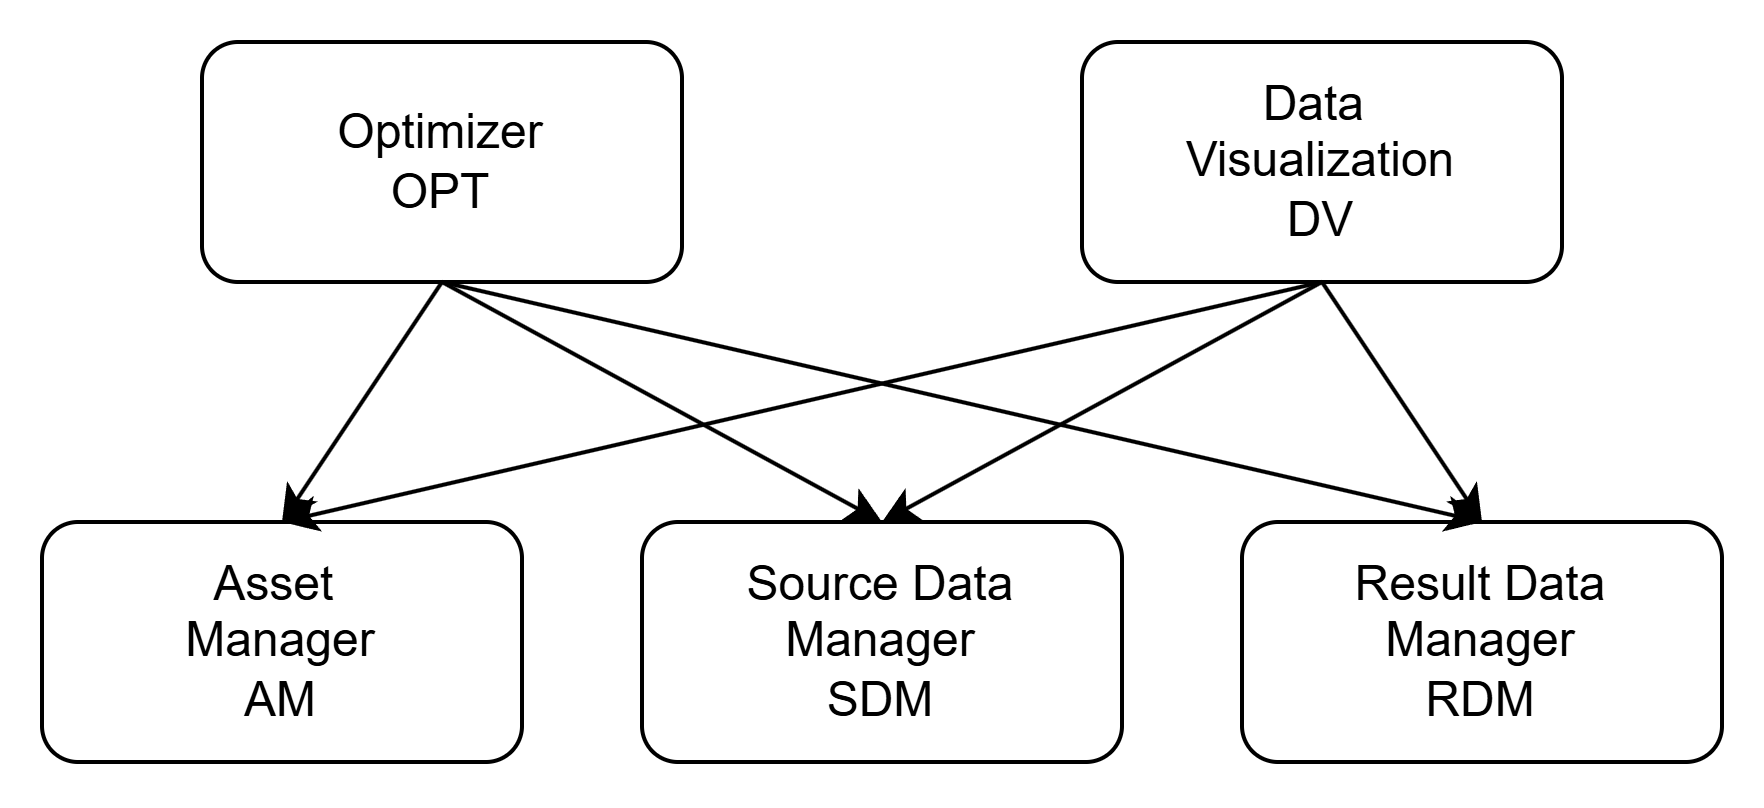
\includegraphics[width=0.8\textwidth]{Images/architecture.png}
    \caption{System Architecture Diagram}
    \label{fig:system-architecture}
\end{figure}

\textbf{Source Data Manager (SDM):}
Serves as a repository for dynamic system information, storing data in local CSV files. The SDM stores and provides two types of data, the amount of heat demanded by the buildings and the current electricity prices, both of which are updated on an hourly basis.

\textbf{Result Data Manager (RDM):}
Scenario 1 operates on a single district heating network with three gas boilers (GB1, GB2, GB3) and one oil boiler (OB1). The gas boilers have lower production costs, while the oil boiler is more expensive and is therefore reserved for peak demand periods. All boilers maintain constant production costs regardless of the hour of operation.
The optimization strategy prioritizes the cheapest gas boiler first, adding output from more expensive units only when needed to meet the total heat demand. One of the gas boilers must also undergo a scheduled maintenance period of between 30 and 60 hours, during which it is taken offline and produces 0 MW.



\subsection*{Scenarios}

\subsubsection*{Scenario 1 (Heat only)}

\hspace*{1cm}Scenario 1 uses a single district heating network with three gas boilers (GB1, GB2, GB3) and one oil boiler (OB1). The gas boilers are cheaper, while the oil boiler has higher production costs and is mainly used in peak demand periods. All boilers have constant production costs that do not depend on the hour of operation. Strategy for scenario one is to run the cheapest gas boiler first and then add production from the more expensive boilers if needed to meet the heat demand. There should also be chosen a period of 30 to 60 hours when one of the gas boilers will be down due to maintenance.

\subsubsection*{Scenario 2 (Heat and electricity)}

\hspace*{1cm}Scenario 2 operates on a network with two gas boilers (GB1, GB3), one gas motor (GM1), and one electric boiler (EB1). The gas motor produces electricity that can be sold on the market, while the electric boiler consumes electricity that must be purchased.
When electricity prices are high, the gas motor is prioritized, as selling electricity generates additional income. When prices are low, the electric boiler becomes the preferred unit, as buying electricity is cheaper. Unit selection is determined each hour by calculating and comparing the net production cost for each unit.


The project is based on data delivered by Danfoss, including:

\begin{itemize}
    \item Graphical representation of the district heating network
    \item Configuration parameters for each production unit (image, produced heat, produced/consumed electricity, primary energy consumption, production costs, CO2 emissions)
    \item Heat demand and electricity prices for a 14-day winter period with 1-hour resolution
    \item Heat demand and electricity prices for a 14-day summer period with 1-hour resolution
\end{itemize}

\medskip

\hspace*{1cm}If there is time left,  project can be extended by usage of other visualization libraries, storing data in a database, enabling or disabling units directly from the UI, running alternative configurations in Scenario 2, and implementing APIs and an API client for reading electricity prices from Energinet.dk.

\section{Functional Requirements}

\hspace*{1cm}The following tables outline the formal functional requirements for the system, translated into standardized system-level behaviors. The requirements are divided into three tables: one for each of the two operational scenarios, and a third covering general app navigation and UI requirements.

\vspace{0.5cm}

% --- TABLE 1: Scenario 1 ---
\renewcommand{\arraystretch}{1.5}
\begin{longtable}{|p{1.5cm}|p{2.4cm}|p{6.7cm}|p{1.4cm}|p{2cm}|}
\caption{Functional Requirements: Scenario 1}
\label{tab:fr_scenario1} \\
\hline
\textbf{ID} & \textbf{Related US} & \textbf{Requirement Description} & \textbf{Priority} & \textbf{Notes} \\
\hline
\endfirsthead

\multicolumn{5}{c}{{\tablename\ \thetable{}: Functional Requirements: Scenario 1}} \\
\hline
\textbf{ID} & \textbf{Related US} & \textbf{Requirement Description} & \textbf{Priority} & \textbf{Notes} \\
\hline
\endhead

\hline \multicolumn{5}{|r|}{{Continued on next page}} \\ \hline
\endfoot

\hline
\endlastfoot

FR-001 & HEAT - 78/79 & The system shall allow the user to input data. & High & SDM\&RDM \\
\hline
FR-002 & HEAT - 78/79 & The system shall allow the user to retrieve input data. & High & SDM\&RDM \\
\hline
FR-003 & HEAT - 79 & The system shall allow the user to output data. & High & Database integration \\
\hline
FR-004 & HEAT - 79 & The system shall allow the user to upload assets from a CSV file. & High & Asset Manager \\
\hline
FR-005 & HEAT - 82 & The system shall allow the user to add an asset. & High & Asset Manager \\
\hline
FR-006 & HEAT - 82 & The system shall allow the user to edit assets. & High & Boiler definitions \\
\hline
FR-007 & HEAT - 188 & The system shall allow the user to restrict the maximum heat output of each unit as follows: GB1 to 3.0 MW, GB2 to 2.0 MW, GB3 to 4.0 MW, and OB1 to 6.0 MW. & Critical & Capacity constraints \\
\hline
FR-008 & HEAT - 146 & The system shall allow the user to schedule the cheapest boilers first to fulfill the district’s heat demand. & Critical & Cost-based dispatch \\
\hline
FR-009 & HEAT - 146 & The system shall prioritize boilers in the following strict order based on production costs: GB1 (510 DKK), GB2 (540 DKK), GB3 (580 DKK), and OB1 (690 DKK). & Critical & Dispatch order \\
\hline
FR-010 & HEAT - 188 & The system shall allow the user to use the more expensive oil boiler (OB1) only to supplement heat during peak demand periods when the gas boilers cannot fulfill the total demand. & High & Peak demand handling \\
\hline
FR-011 & HEAT - 188 & The system shall allow the user to optimize units separately for both a winter period and a summer period. & High & Seasonal optimization \\
\hline
FR-012 & HEAT - 146 & The system shall remove a designated gas boiler from the available pool of units during its scheduled maintenance period, ensuring it produces 0 MW. & Medium & Maintenance logic \\
\hline
FR-013 & HEAT - 146 & The system shall validate that the user’s selected maintenance duration is a minimum of 30 hours and a maximum of 60 hours. & Medium & Maintenance validation \\
\hline
FR-014 & HEAT - 147/148 & The system shall display a chart or graph that visually compares the total heat demand against the individual heat output contributions of GB1, GB2, GB3, and OB1 over time. & High & Result graphing \\
\hline
FR-015 & HEAT - 188 & The system shall allow the user to choose an obligatory maintenance period for one unit in both the summer and winter periods. & Medium & Maintenance scheduling \\
\end{longtable}


% --- TABLE 2: Scenario 2 ---
\begin{longtable}{|p{1.5cm}|p{2.4cm}|p{6.7cm}|p{1.4cm}|p{2cm}|}
\caption{Functional Requirements: Scenario 2}
\label{tab:fr_scenario2} \\
\hline
\textbf{ID} & \textbf{Related US} & \textbf{Requirement Description} & \textbf{Priority} & \textbf{Notes} \\
\hline
\endfirsthead

\multicolumn{5}{c}{{\tablename\ \thetable{}: Functional Requirements: Scenario 2}} \\
\hline
\textbf{ID} & \textbf{Related US} & \textbf{Requirement Description} & \textbf{Priority} & \textbf{Notes} \\
\hline
\endhead

\hline \multicolumn{5}{|r|}{{Continued on next page}} \\ \hline
\endfoot

\hline
\endlastfoot

FR-016 & HEAT - 40/91/92 & The system shall allow the user to retrieve hourly electricity prices data from the database. & High & SDM\&RDM \\
\hline
FR-017 & HEAT - 91/92 & The system shall allow the user to retrieve hourly heat demand data from the database. & High & Market data retrieval \\
\hline
FR-018 & HEAT - 79/277 & The system shall allow the user to upload assets from a CSV file. & High & Unit registration \\
\hline
FR-019 & HEAT - 146 & The system shall allow the user to limit the maximum heat output of each unit: GB1 to 3.0 MW, GB3 to 4.0 MW, GM1 to 5.3 MW, and EB1 to 6.0 MW. & High & Heat capacity constraints \\
\hline
FR-020 & HEAT - 146 & The system shall allow the user to account for electricity production and consumption capacities, specifically noting that GM1 produces up to 3.9 MW of electricity, while EB1 consumes up to 6.0 MW (-6.0 MW). & High & Electricity constraints \\
\hline
FR-021 & HEAT - 188/203 & The system shall allow the user to calculate the net production costs for the electricity-producing/consuming units based on fluctuating electricity prices. & High & Dynamic net cost calculation \\
\hline
FR-022 & HEAT - 188 & The system shall prioritize running the gas motor (GM1) during periods of high electricity prices. & Critical & High-price optimization logic \\
\hline
FR-023 & HEAT - 188 & The system shall prioritize running the electric boiler (EB1) during periods of low electricity prices. & Critical & Low-price optimization logic \\
\hline
FR-024 & HEAT - 188 & The system shall actively prevent the gas motor (GM1) from running during summer periods with negative electricity prices (to avoid paying for produced electricity). & Critical & OPT \\
\hline
FR-025 & HEAT - 188 & The system shall recognize the electric boiler as an extra income source during negative price hours. & High & Negative price handling \\
\hline
FR-026 & HEAT - 146 & The system shall completely remove either GB1 or GM1 from the optimization calculations during its scheduled maintenance period. & High & Maintenance logic \\
\hline
FR-027 & HEAT - 146 & The system shall allow the user to select an obligatory maintenance period for either GB1 or GM1, and enforce a duration between 30 and 60 hours. & Medium & Maintenance scheduling \\
\hline
FR-028 & HEAT - 146 & The system shall display a graph comparing the total heat demand against the individual heat output contributions of GB1, GB3, GM1, and EB1 over time. & Medium & Result graphing \\
\end{longtable}


% --- TABLE 3: General App Navigation and UI ---
\begin{longtable}{|p{1.5cm}|p{2.4cm}|p{6.7cm}|p{1.4cm}|p{2cm}|}
\caption{Functional Requirements: General App Navigation \& UI.}
\label{tab:fr_general} \\
\hline
\textbf{ID} & \textbf{Related US} & \textbf{Requirement Description} & \textbf{Priority} & \textbf{Notes} \\
\hline
\endfirsthead

\multicolumn{5}{c}{{\tablename\ \thetable{} -- continued from previous page}} \\
\hline
\textbf{ID} & \textbf{Related US} & \textbf{Requirement Description} & \textbf{Priority} & \textbf{Notes} \\
\hline
\endhead

\hline \multicolumn{5}{|r|}{{Continued on next page}} \\ \hline
\endfoot

\hline
\endlastfoot

FR-029 & HEAT - 149 & Upon launch, the system shall display a home screen allowing the user to explicitly select between Scenario 1 and Scenario 2. & High & Startup Page \\
\hline
FR-030 & HEAT - 149 & The system shall allow the user to easily navigate between scenarios. & High & Scenario navigation \\
\hline
FR-031 & HEAT - 91/92/233 & The system shall allow the user to use a database system to save and retrieve data. & High & Database storage \\
\hline
FR-032 & HEAT - 84/85 & The system shall allow the user to dynamically activate or deactivate individual heating units from being considered in the optimizer’s calculations. & High & Dynamic unit toggling \\
\hline
FR-033 & HEAT - 84 & The system shall allow the user to run a custom scenario with configurations set by the user. & High & Custom scenario configuration \\
\hline
FR-034 & HEAT - 147/188 & The system shall provide results of different configured scenarios for result comparison. & High & Comparison metrics \\
\end{longtable}

\newpage
\section{Non-Functional Requirements}

\hspace*{1cm}The following table details the non-functional requirements (NFRs), which define the system's quality attributes, performance standards, and operational constraints.

\vspace{0.5cm}

% --- TABLE 4: Non-Functional Requirements ---
\begin{longtable}{|p{2cm}|p{8cm}|p{4cm}|}
\caption{Non-Functional Requirements detailing system quality attributes.}
\label{tab:non_functional_requirements} \\
\hline
\textbf{ID} & \textbf{Requirement Description} & \textbf{Notes} \\
\hline
\endfirsthead

\multicolumn{3}{c}{{\tablename\ \thetable{}: Non-Functional Requirements detailing system quality attributes.}} \\
\hline
\textbf{ID} & \textbf{Requirement Description} & \textbf{Notes} \\
\hline
\endhead

\hline \multicolumn{3}{|r|}{{Continued on next page}} \\ \hline
\endfoot

\hline
\endlastfoot

NFR-001 & The system shall complete all optimization calculations within 3 seconds of the user clicking 'Optimize'. & Optimization speed \\
\hline
NFR-002 & The system shall completely render the resulting graphs within 3 seconds of the user clicking 'Optimize'. & Processing speed \\
\hline
NFR-003 & The system shall efficiently load, process, and aggregate a full month of hourly data (approximately 720-744 data points) without UI freezing or lag. & Data volume handling \\
\hline
NFR-004 & The system shall be fully cross-platform compatible, executing reliably on Windows, macOS, and Linux operating systems. & Cross-platform compatibility \\
\hline
NFR-005 & The system shall present the entire user interface, including all menus, labels, and error messages, in English. & UI Language \\
\hline
NFR-006 & The system shall calculate and display all financial values, production costs, and revenues strictly using Danish Kroner (DKK). & Currency localization \\
\hline
NFR-007 & The system shall generate a highly readable visualization for a month of data, formatting the daily boiler usage as a stacked chart (matching the total heat demand on the Y-axis, and days of the month on the X-axis) alongside a daily cost graph. & Visualization clarity \\
\hline
NFR-008 & The system shall not crash if user loses their internet connection. & System stability \\
\hline
NFR-009 & The system shall handle API failures by displaying a clear, understandable error feedback message or popup to the user. & Exception handling \\
\end{longtable}

\section{System Requirements}
\hspace*{1cm}The system is split into three parts: Front End, Back End and the Database. Both the Backend and the Database are run in a Linux Docker container. The Frontend is run locally on the user's machine. For a machine to run the project they need the following:

\subsection*{Software Specifications}
\begin{description}
    \item[Entire project:] .NET 9.0
    \item[Backend:] Docker Desktop (latest version)
    \item[Database:] Docker Desktop with MySql Image (shall be installed automatically if missing)
    \item[Frontend:] Required NuGet packages (all must be compatible with .NET 9.0):
    \begin{itemize}
        \item Avalonia.UI
    \end{itemize}
\end{description}
                             

\chapter[Scrum Implementation]{Scrum Implementation}             
\label{chap:scrum}                                            
% -------------------------------------------------------------
% SCRUM IMPLEMENTATION
% -------------------------------------------------------------
\section{Scrum Implementation}

\hspace*{1cm}The team implemented SCRUM and its ceremonies from the very first week of development. Two week long sprints were used for the whole duration of development. However, there were certain changes throughout the semester based on team's experience in order to optimize team's workflow.

\medskip

\hspace*{1cm}Scrum master was elected in the beginning and due to his effectivity he was in this role until the end of this project. All team members agreed on using Jira. Jira was chosen because it allowed the team to use all features such as task management and proper story point assignment without the need of additional subscriptions. Jira proved to be a good fit, because it is better optimized for bigger projects the team found it very helpful. Backlog was used for storing future tasks, from backlog certain tasks were taken to sprint backlog during sprint plannings. Board for each sprint consisted of several columns, “TO DO”, “IN PROGRESS”, “UNIT TESTING”, “UNDER REVIEW” and “DONE”. One member connected Jira seamlessly with IDEs, so when a team member started on a new branch the task would automatically move to “IN PROGRESS”. Very important aspect of team cooperation was the approach to reviews. Every task required a minimum of two reviewers. If a reviewer found something imperfect, a change request was created in GitHub and the branch owner had to fix it before the reviewer would approve it again.

\medskip

\hspace*{1cm}Project was finished in 6 sprints. Each sprint consisted of necessary ceremonies. Our team decided to have two standup meetings, one in each week of the two week sprint, usually on Mondays and Wednesdays. Standup meetings were short, structured and valuable part of our communication throughout the semester and they stayed unchanged until the end.

\medskip
\medskip

\hspace*{1cm}Sprint plannings were held every other week before the start of a new sprint. Four hour block was determined to this ceremony every single time. For the first two sprints plannings were held on Mondays. After this period team decided to move sprint planning to Friday the week before. Monday was particularly busy day for all team members and moving sprint planning to Friday had the benefit of one more weekend, so it essentially prolonged the sprint period. With each new sprint planning less time was needed as the team members understood and got better in planning, focusing and critically thinking about what needs to be done and who is the correct person for specific task.

\medskip

\hspace*{1cm}At the end of each sprint team held two last ceremonies. Sprint review and sprint retrospective. Both of these ceremonies were held on Fridays. 

\hspace*{1cm}Originally, all deadlines for tasks and pull-request reviews were set for Thursday evening. However, the team found this really ineffective and there was not enough time for reviews to be done. The deadline for tasks was later moved to Wednesdays evening and reviews deadline to Thursdays evening, so there would be enough time for all ceremonies held on Friday. 

\hspace*{1cm}In sprint review team members stated what each of them accomplished and how they felt about it. This ceremony was especially important for the team as it provided information about what each member prefers, what is their level at certain tasks and it allowed everyone to understand what exactly and how things were done in the past two weeks. Sprint retrospective was done through Jira. For each sprint one team member created a table with three columns “Start doing”, “Stop doing” and “Keep doing”. After ten minutes of anonymous answering team members checked and talked about the topics in the table. This turned out to be as helpful as sprint review. Retrospective was definitely the ceremony that contributed the most to team's growth and ability to cooperate effectively.
                             

\chapter[Sprints]{Sprints}             
\label{chap:sprints}                                            
% -------------------------------------------------------------
% SPRINTS
% -------------------------------------------------------------

\section{Sprint 1}
\textbf{Goal:} First sprint focusing on the beginning of the project, including report writing and initial coding tasks.

\medskip
\noindent \textbf{Short summary:} Both report and coding tasks were completed successfully. 2 bugs were not fixed. On report
entity framework still persisted. During this sprint the team realized the importance of correct story point assignment and the need for better communication between team members. The retrospective revealed that the team needs to improve on time management and task estimation for future sprints (Sprint 1 planning, backlog, and retrospective can be found in Appendix \ref{appendix:figures}).

\section{Sprint 2}

\medskip
\noindent \textbf{Short summary:} This sprint there were no report tasks. On the other hand the team made good progress on the code side,
getting closer to the first feasable demo. All tasks were successfully finished. Unit tests were written retroactively to Asset/Source services. The frontend was connected to the backend and Results/ResultLists were created. 
This sprint the team started experimenting with user stories that could not be finished in one sprint, because of significant complexity.
In cases like this subtasks were assigned as if they were normal tasks. These large items were left in TODO for each sprint until all
subtasks were done. Team members started figuring out the optimizing algorithm used by the system, and created the Asset Manager Window (Sprint 2 planning, backlog, and retrospective can be found in Appendix \ref{appendix:figures}).

\section{Sprint 3}
\textbf{Goal:} Third sprint focusing on the completion of the first demo, including the implementation of the optimization algorithm and the creation of a user interface.

\medskip
\noindent \textbf{Short summary:} The team managed to complete all required tasks for the demo, even though one task had to be left 
for the next sprint, as it was not necessary for the demo and it took up precious time from 
working on the demo. Minor tasks had to be assigned in the middle of the sprint. For example CSV creation for the demo was not planned, but it was necessary to show the results of optimization (Sprint 3 planning, backlog, and retrospective can be found in Appendix \ref{appendix:figures}).

\section{Sprint 4}
\textbf{Goal:} Fourth sprint focusing on LaTex report writing and implementing feedback received from the midterm evaluation.

\medskip
\noindent \textbf{Short summary:} The team managed to implement most of the feedback received on the midterm evaluation and the project
is wrapping up nicely. Members are going to focus on implementing extra 
requirements. Report got migrated from Word over to LaTeX so the team focused more on fitting it to the given template (Sprint 4 planning, backlog, and retrospective can be found in Appendix \ref{appendix:figures}).

\section{Sprint 5}
\textbf{Goal:} Fifth sprint focusing on report tasks as well as on small quality of life UI changes.

\medskip
\noindent \textbf{Short summary:} The first week of this sprint was unfortunate as not all team members were in Denmark and could not fully concentrate. Despite the short time, the team managed to implement all tasks preparing for final 
sprint. Except for merge conflicts slipping through and making the main branch not 
working, there were not any big problems (Sprint 5 backlog and retrospective can be found in Appendix \ref{appendix:figures}).

\section{Sprint 6}
\textbf{Goal:} Sixth sprint focusing on report and code finalization.

\medskip
\noindent \textbf{Short summary:} The team managed to finish all tasks for the final sprint, including report finalization and code cleanup. Overall, the project was a success and the team is proud of what they have accomplished (Sprint 6 planning and retrospective can be found in Appendix \ref{appendix:figures}).
                             

\chapter[Solution (Technical Aspect)]{Solution (Technical Aspect)}             
\label{chap:solution}                                            
% -------------------------------------------------------------
% SOLUTION(TECHNICAL ASPECT)
% -------------------------------------------------------------
\noindent 

\hspace*{1cm}This chapter outlines the steps undertaken to achieve the final solution, starting from the project description, describing the technical architecture in the process. The development process began with going through the provided Project Description, and rewriting it into a shorter version, keeping only the most important parts. The compact version was suitable for conducting the verb/noun analysis where class and method candidates emerged. The class candidates are able to be transformed into CRC cards outlining the responsibilities and collaborators of each class. The CRC cards are used to provide UML diagrams(Class,Package,Activity and Sequence).

\section{Verb-noun analysis}

\hspace*{1cm}\textcolor{nounred}{Asset Manager (AM)} should \textcolor{verbblue}{store} its \textcolor{nounred}{data} in local \textcolor{nounred}{files} and \textcolor{verbblue}{supply} other \textcolor{nounred}{modules} with it. \textcolor{nounred}{Source Data Manager (SDM)} should \textcolor{verbblue}{store} \textcolor{nounred}{dynamic data} in \textcolor{nounred}{csv files}. \textcolor{nounred}{Result Data Manager (RDM)} should \textcolor{verbblue}{save} \textcolor{nounred}{result data} in local \textcolor{nounred}{CSV files}. \textcolor{nounred}{Optimizer (OPT)} should \textcolor{verbblue}{calculate} the best \textcolor{nounred}{economical schedule} of the \textcolor{nounred}{heat production} for a given \textcolor{nounred}{period}. It also \textcolor{verbblue}{secures} \textcolor{nounred}{heat availability} to all \textcolor{nounred}{buildings} at any \textcolor{nounred}{time}. There are different \textcolor{nounred}{units}, each \textcolor{verbblue}{has} a specific \textcolor{nounred}{production cost}, expressed in \textcolor{nounred}{DKK} per MWh produced \textcolor{nounred}{heat}. For \textcolor{nounred}{heat only units} there are no further \textcolor{nounred}{expenses} nor \textcolor{nounred}{income}. \textcolor{nounred}{Electricity producing units} should \textcolor{verbblue}{sell} the produced \textcolor{nounred}{electricity} and \textcolor{verbblue}{have} thereby an extra \textcolor{nounred}{income} depending on the \textcolor{nounred}{electricity prices} which can \textcolor{verbblue}{change} from \textcolor{nounred}{hour} to \textcolor{nounred}{hour}. \textcolor{nounred}{Electricity consuming units} should \textcolor{verbblue}{buy} the \textcolor{nounred}{electricity} and \textcolor{verbblue}{have} thereby an extra \textcolor{nounred}{expense}, again depending on the \textcolor{nounred}{electricity prices}. \textcolor{nounred}{Net production cost} should be \textcolor{verbblue}{calculated} differently for each \textcolor{nounred}{unit type} and \textcolor{verbblue}{compared} to build \textcolor{nounred}{priorities}. The \textcolor{nounred}{Data Visualization} should \textcolor{verbblue}{display} a \textcolor{nounred}{graphical presentation} of important \textcolor{nounred}{source and result data}.

\vspace{2em}

\subsection*{\textcolor{nounred}{Candidates for classes:}}
\begin{multicols}{3} % splits the list into 3 columns
\begin{itemize}
    \item Asset Manager
    \item Data
    \item Files
    \item Modules
    \item Source Data Manager
    \item Result Data Manager
    \item Optimizer
    \item Schedule
    \item Production
    \item Period
    \item Heat availability
    \item Buildings
    \item Time
    \item Electricity
    \item Units (GB1-EB1)
    \item Income
    \item Expenses
    \item Prices
    \item Net production cost
    \item Unit type
    \item Data Visualization
    \item Presentation
    \item Priorities
\end{itemize}
\end{multicols}

\vspace{2em}

\subsection*{\textcolor{verbblue}{Candidates for methods:}}
\begin{multicols}{3}
\begin{itemize}
    \item Store
    \item Supply
    \item Save
    \item Calculate
    \item Secures
    \item Has
    \item Sell
    \item Have
    \item Depending
    \item Change
    \item Buy
    \item Compare
    \item Display
\end{itemize}
\end{multicols}

\vspace{2em}

\section{Classes and Methods Mapping}
\renewcommand{\arraystretch}{1.5} % adds vertical padding to rows
\begin{tabularx}{\textwidth}{@{} l X @{}}
    \toprule
    \textbf{Class Name} & \textbf{Associated Methods} \\
    \midrule
    \textcolor{nounred}{AssetManager} & \textcolor{verbblue}{store}, \textcolor{verbblue}{supply} \\
    \textcolor{nounred}{SourceDataManager} & \textcolor{verbblue}{store} (dynamic data), \textcolor{verbblue}{read} CSV \\
    \textcolor{nounred}{ResultDataManager} & \textcolor{verbblue}{save} (results) \\
    \textcolor{nounred}{Optimizer} & \textcolor{verbblue}{calculate} (schedule), \textcolor{verbblue}{secure} (heat availability), \textcolor{verbblue}{compare} \\
    \textcolor{nounred}{Unit} & \textcolor{verbblue}{sell} (electricity), \textcolor{verbblue}{buy} (electricity), \textcolor{verbblue}{calculate} net production cost \\
    \textcolor{nounred}{DataVisualization} & \textcolor{verbblue}{display} (graphical data) \\
    \bottomrule
\end{tabularx}

\subsection*{CRC Cards}
% Asset Manager Card
\noindent
\begin{tabularx}{\textwidth}{| X | X |}
    \hline
    \multicolumn{2}{| p{\dimexpr\textwidth-2\tabcolsep-2\arrayrulewidth}|}{\textbf{Class:} \textcolor{nounred}{Asset Manager}} \\
    \hline
    \textbf{Responsibilities} & \textbf{Collaborators} \\
    \hline
    \begin{itemize}[leftmargin=*, nosep, before=\vspace{-0.2\baselineskip}]
        \item Store heater data
    \end{itemize} & 
    \begin{itemize}[leftmargin=*, nosep, before=\vspace{-0.2\baselineskip}]
        \item Optimizer
        \item Data Visualization
        \item Unit
    \end{itemize} \\
    \hline
\end{tabularx}

\vspace{1.5em} % Space between cards

% Optimizer Card
\noindent
\begin{tabularx}{\textwidth}{| X | X |}
    \hline
    \multicolumn{2}{| p{\dimexpr\textwidth-2\tabcolsep-2\arrayrulewidth}|}{\textbf{Class:} \textcolor{nounred}{Optimizer}} \\
    \hline
    \textbf{Responsibilities} & \textbf{Collaborators} \\
    \hline
    \begin{itemize}[leftmargin=*, nosep, before=\vspace{-0.2\baselineskip}]
        \item Calculates heating schedule
    \end{itemize} & 
    \begin{itemize}[leftmargin=*, nosep, before=\vspace{-0.2\baselineskip}]
        \item Asset Manager
        \item Source Data Manager
        \item Result Data Manager
    \end{itemize} \\
    \hline
\end{tabularx}

\vspace{1.5em}

% Source Data Manager Card
\noindent
\begin{tabularx}{\textwidth}{| X | X |}
    \hline
    \multicolumn{2}{| p{\dimexpr\textwidth-2\tabcolsep-2\arrayrulewidth}|}{\textbf{Class:} \textcolor{nounred}{Source Data Manager}} \\
    \hline
    \textbf{Responsibilities} & \textbf{Collaborators} \\
    \hline
    \begin{itemize}[leftmargin=*, nosep, before=\vspace{-0.2\baselineskip}]
        \item Stores market data
    \end{itemize} & 
    \begin{itemize}[leftmargin=*, nosep, before=\vspace{-0.2\baselineskip}]
        \item Optimizer
        \item Data Visualization
    \end{itemize} \\
    \hline
\end{tabularx}

\vspace{1.5em}

% Result Data Manager Card
\noindent
\begin{tabularx}{\textwidth}{| X | X |}
    \hline
    \multicolumn{2}{| p{\dimexpr\textwidth-2\tabcolsep-2\arrayrulewidth}|}{\textbf{Class:} \textcolor{nounred}{Result Data Manager}} \\
    \hline
    \textbf{Responsibilities} & \textbf{Collaborators} \\
    \hline
    \begin{itemize}[leftmargin=*, nosep, before=\vspace{-0.2\baselineskip}]
        \item Save output data
    \end{itemize} & 
    \begin{itemize}[leftmargin=*, nosep, before=\vspace{-0.2\baselineskip}]
        \item Data Visualization
        \item Optimizer
    \end{itemize} \\
    \hline
\end{tabularx}

\vspace{1.5em}

% Data Visualization Card
\noindent
\begin{tabularx}{\textwidth}{| X | X |}
    \hline
    \multicolumn{2}{| p{\dimexpr\textwidth-2\tabcolsep-2\arrayrulewidth}|}{\textbf{Class:} \textcolor{nounred}{Data Visualization}} \\
    \hline
    \textbf{Responsibilities} & \textbf{Collaborators} \\
    \hline
    \begin{itemize}[leftmargin=*, nosep, before=\vspace{-0.2\baselineskip}]
        \item Display important data to the user
    \end{itemize} & 
    \begin{itemize}[leftmargin=*, nosep, before=\vspace{-0.2\baselineskip}]
        \item Source Data Manager
        \item Result Data Manager
        \item Asset Manager
    \end{itemize} \\
    \hline
\end{tabularx}

\vspace{1.5em}

% Units Card
\noindent
\begin{tabularx}{\textwidth}{| X | X |}
    \hline
    \multicolumn{2}{| p{\dimexpr\textwidth-2\tabcolsep-2\arrayrulewidth}|}{\textbf{Class:} \textcolor{nounred}{Units}} \\
    \hline
    \textbf{Responsibilities} & \textbf{Collaborators} \\
    \hline
    \begin{itemize}[leftmargin=*, nosep, before=\vspace{-0.2\baselineskip}]
        \item Contains data for different heaters
        \item Calculate net production costs
    \end{itemize} & 
    \begin{itemize}[leftmargin=*, nosep, before=\vspace{-0.2\baselineskip}]
        \item Optimizer
        \item Asset Manager
    \end{itemize} \\
    \hline
\end{tabularx}

\vspace{2em}

\section{System Design}
\noindent The system design, implementing the five modules(OPT,DV,AM,SDM and RDM), focuses on distinguishing data, services and the presentation layer. This was achieved by storing data in a Database, having a Backend API for services and a Frontend UI for the presentation layer. The layering helps create a modular solution, that is able to implement every module in a logical way, without affecting one another.
\subsection{UML Diagram - Class Diagram}
\begin{figure}[H]
    \centering
    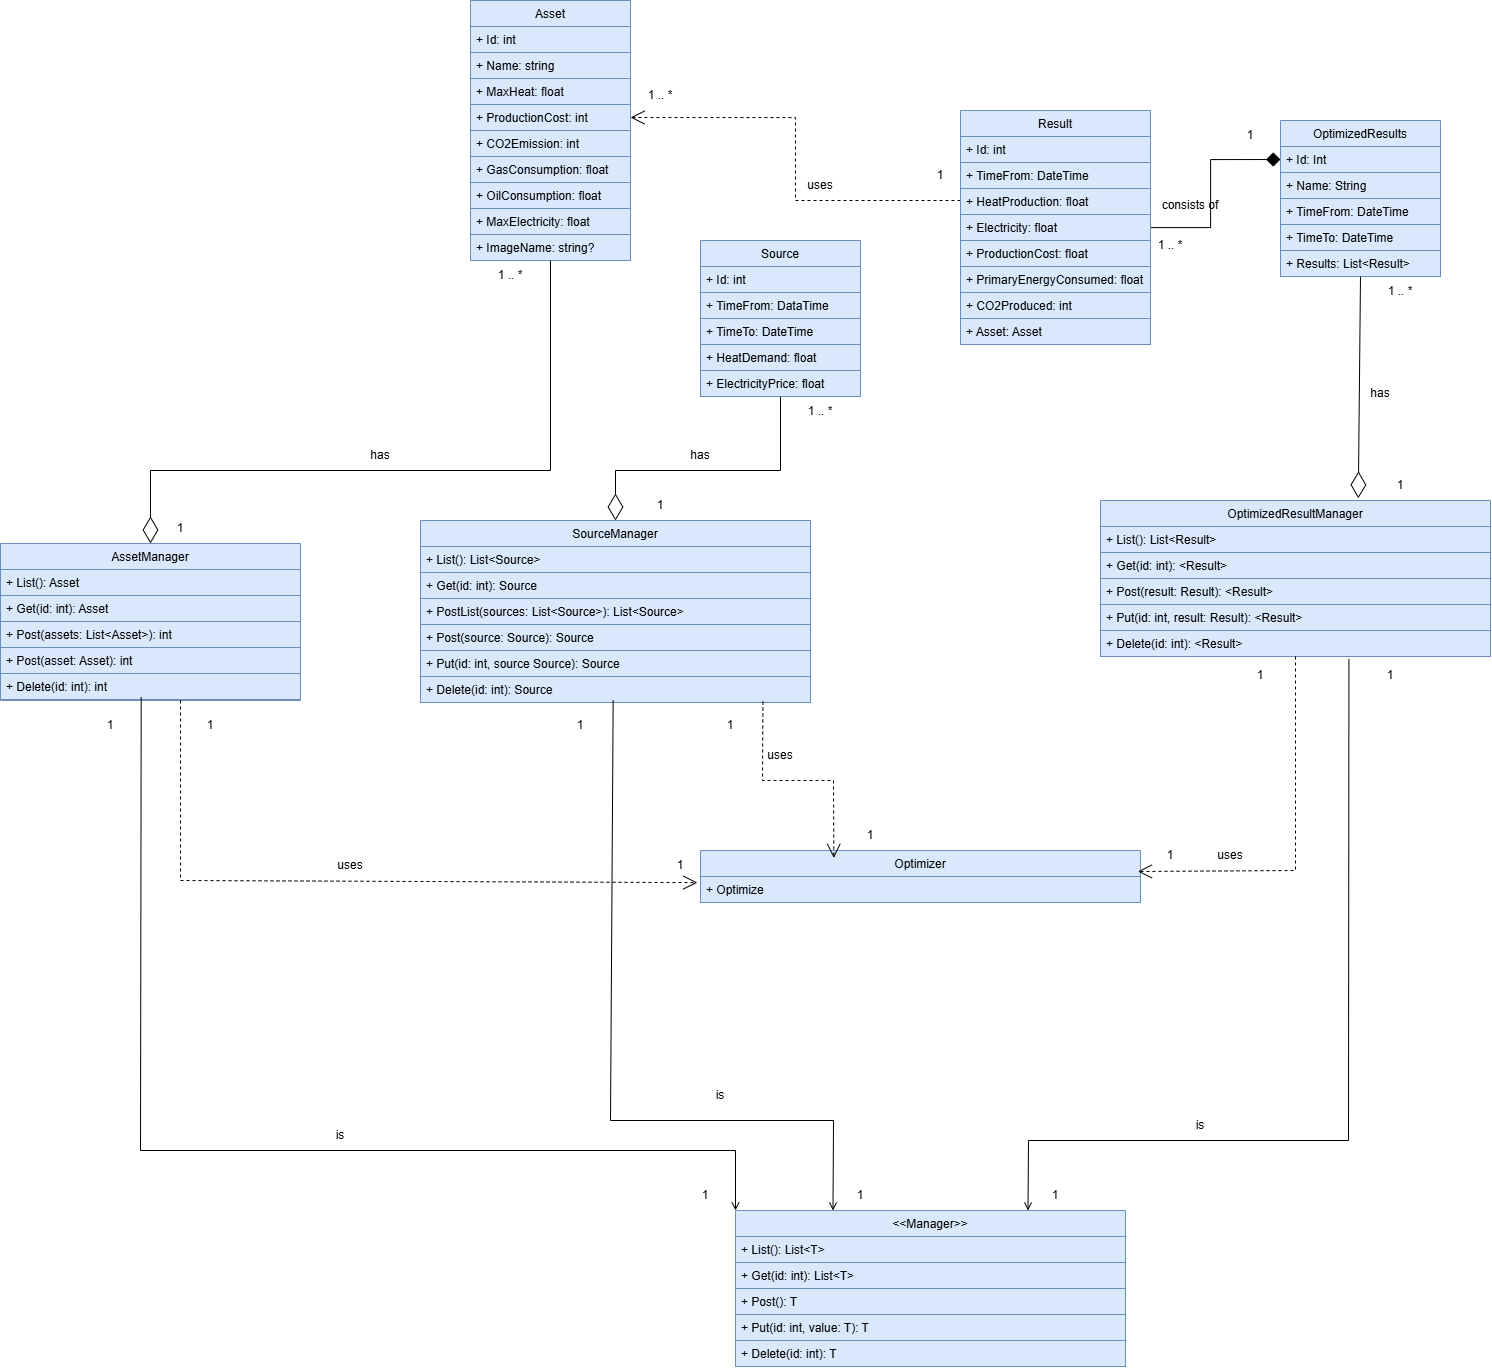
\includegraphics[width=0.9\textwidth]{Images/UML.png} 
    \caption{HeatItOn Abstract Class UML Diagram}
    \label{fig:system_uml}
\end{figure}
\noindent The diagram (Figure~\ref{fig:system_uml}) represents the unified system architecture. This is an abstract version that simplifies the structure down to core components, on which the system is based on. The simplicity of the UML helps with understanding the overall structure of the system, while showing all major classes. 
\subsection{UML Diagram - Package Diagram}
\begin{figure}[H]
    \centering
    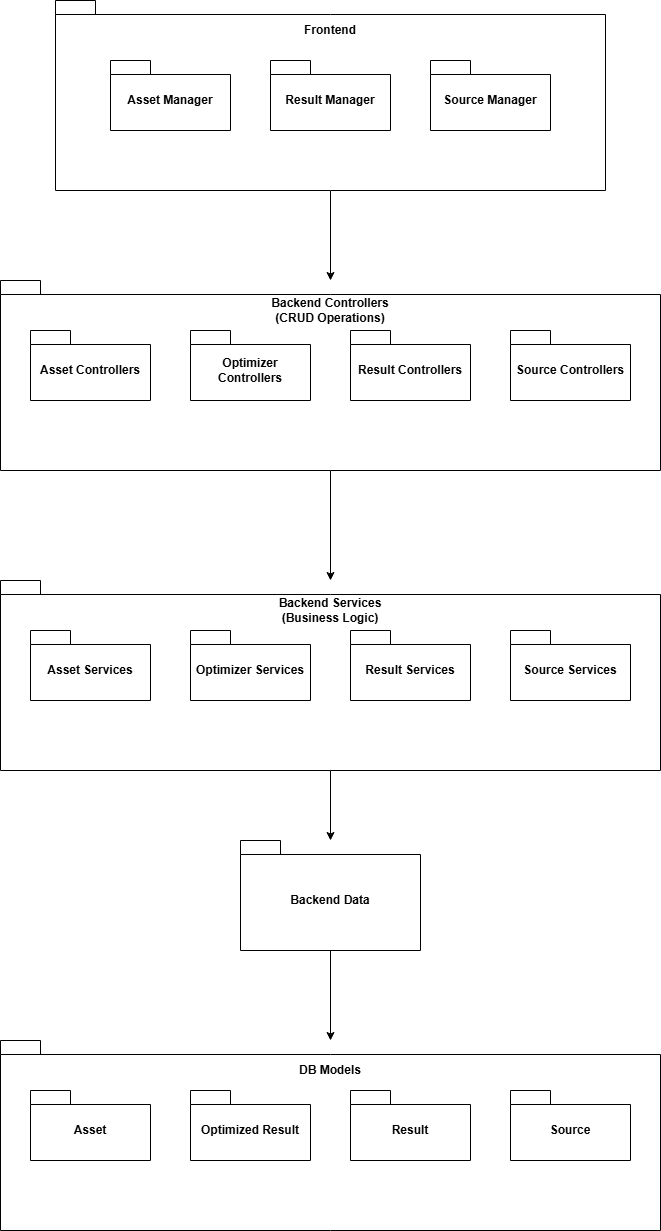
\includegraphics[width=0.8\textwidth]{Images/HeatItOn-Package-Diagram.png} 
    \caption{Package UML Diagram - Five main packages of the system.}
    \label{fig:package_uml}
\end{figure}

The package diagram shown (Figure~\ref{fig:package_uml}) simplified the system into five packages. 

The first one is the Frontend package, containing the Asset, Result and Source Managers. This is the UI of the system, with what the user will interact. The Frontend is following the Model-View-ViewModel pattern, layering the different parts of each manager. This package connects with the next package through clients.

The second package, the Backend Controllers, contain the CRUD(Create, Read, Update, Delete) operations of each module. Through HTTP requests these can be accessed and will call the services in the next package.

Backend Services are the third package containing all the business logic (like the Optimization algorithm).

The forth package is the connection with the Database. It is stored in the Data layer of the Backend. The role of the package is to allow communication between the services and the Database.

The fifth and final package consists of the DB Models(Asset, Source, Result) that are stored in the Database.

This diagram shows a very simplified relationship with the most important parts of the overall system, giving an understanding of the overall workings and layers. Although it is very simple, it is a good starting point for understanding the entire architecture.

The five packages are the backbone of the implementation. Allthough they are much more detailed, this simplified version helps understanding the workings of the solution.

\subsection{UML Diagram - Activity Diagram (Add Asset)}
\begin{figure}[H]
    \centering
    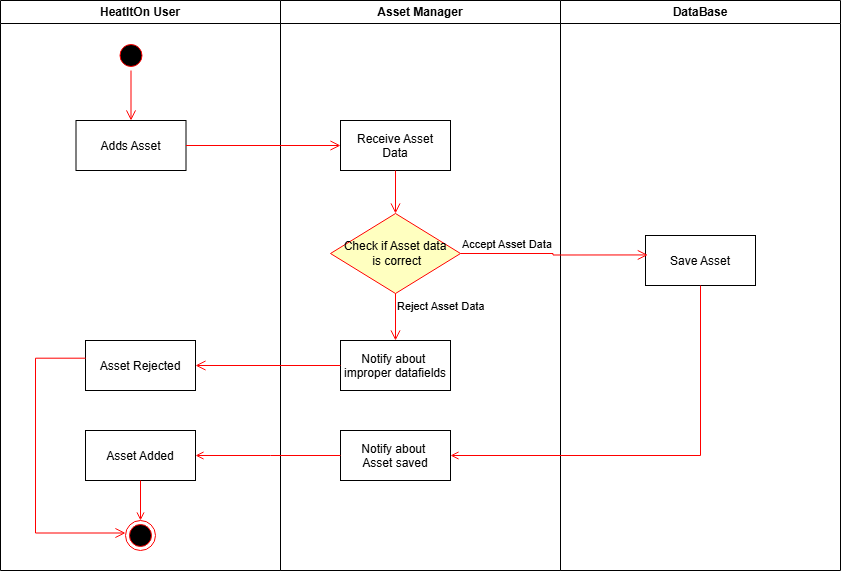
\includegraphics[width=0.9\textwidth]{Images/HeatItOn_activity_diagram_add_asset.png} 
    \caption{Add Asset Activity UML Diagram - Three parts and their actions for adding a new Asset.}
    \label{fig:add_asset_uml}
\end{figure}
The activity UML diagram (Figure~\ref{fig:add_asset_uml}) depicts the addition of a new Asset by the user into the system.

The activity is initiated by the user when they want to add a new Asset interacting with the Asset Manager. The filled out data is then verified by the Asset Manager. If the data was filled out correctly (like having a proper name or number fields having numbers) the Asset Manager will create the Asset and send it to the Database, who will save it. If the data was not filled out correctly, it will reject the received data. The activity ends with the user being notified of both cases, ending it. For a successful addition the Asset Manager will also display the new Asset instantly.

Adding an Asset is started in the Frontend. The Frontend clients will call the Backend that will handle the communication with the Database where the Asset will be saved. The Frontend deals with user input and handling the data as well.

This diagram helps getting an idea about how the communication, for adding Assets, works. This activity is crucial to the solution, as every Asset needs to be stored in the Database for the optimization to work.

\subsection{UML Diagram - Activity Diagram (Import Sources)}
\begin{figure}[H]
    \centering
    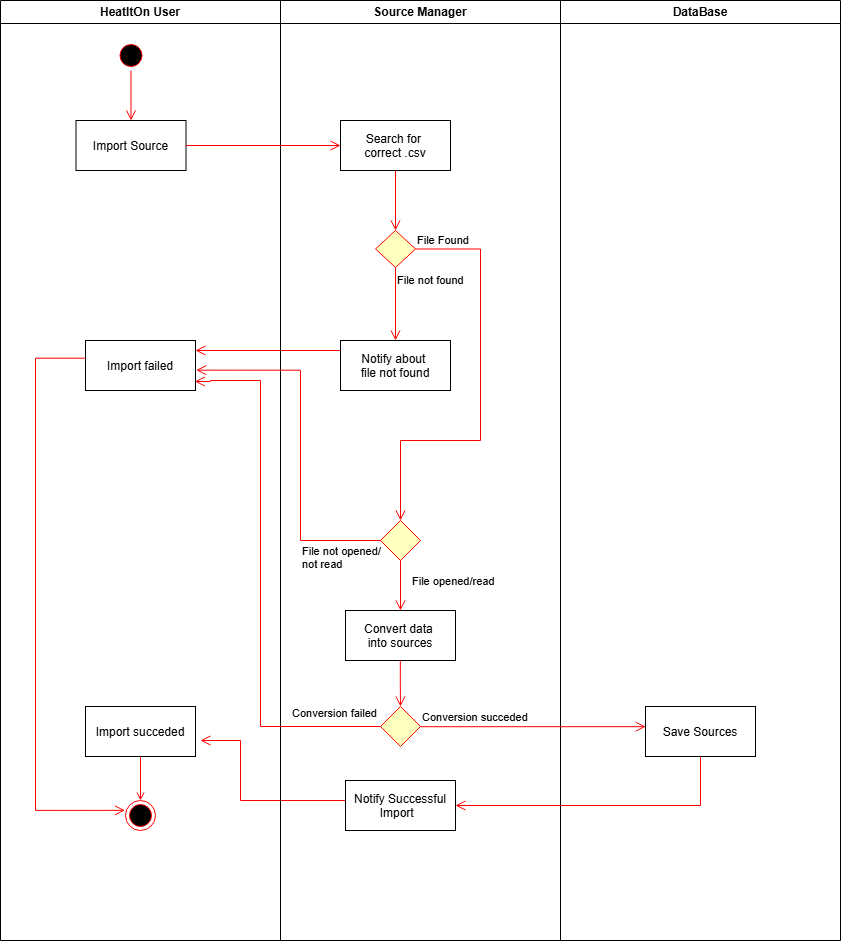
\includegraphics[width=0.9\textwidth]{Images/HeatItOn_activity_diagram_import_source.png} 
    \caption{Import Sources Activity UML Diagram - Three parts and their actions for importing Sources from a csv file.}
    \label{fig:import_sources_uml}
\end{figure}

The activity UML diagram (Figure~\ref{fig:import_sources_uml}) depicts the importing of one or multiple Sources stored in a Comma Separated Value(csv) file. 

Importing is initiated by the user interacting with the Source Manager UI. The Source Manager then will try to find the requested csv file. If the file is found the Source Manager will try to open and read the data in the Frontend. After a successful opening and reading the data will be transformed into proper Source models and will be sent over through the Backend to the Database for storage, notifying the user. If the file is not found or if the file cannot be opened or read properly, like if the csv is not structured properly, the importing process fails and the user is notified. The activity is concluded by notifying the user of either a successful or failed import, the former is visible by a new data set appearing in the Source Manager.

This helps getting an understanding of how importing works for sources (but not only), and the workings of the Source Manager.

The Source Manager and Sources are the other crucial part of the system, without which, the optimization process could not be run.

\subsection{UML Diagram - Activity Diagram (Delete Asset)}
\begin{figure}[H]
    \centering
    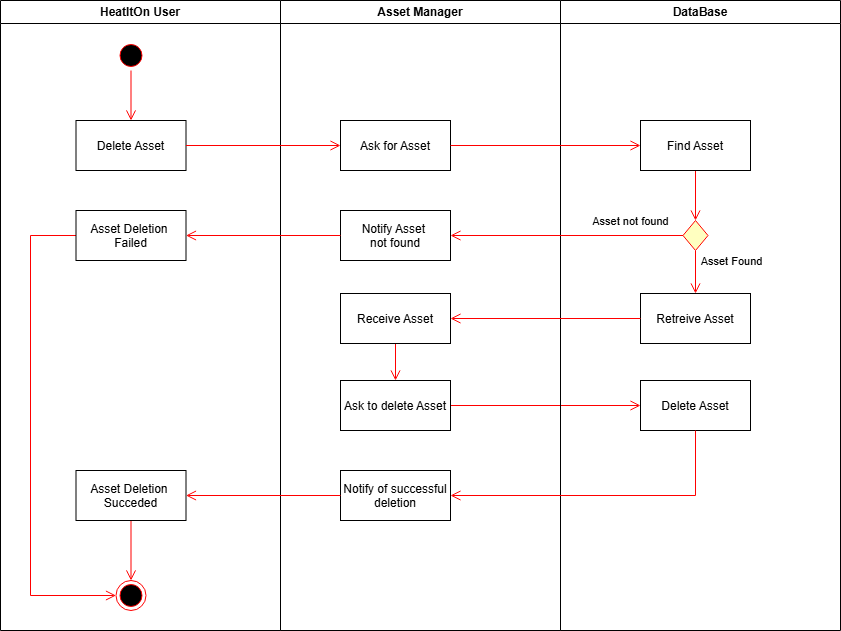
\includegraphics[width=0.9\textwidth]{Images/HeatItOn_activity_diagram_delete_asset.png} 
    \caption{Delete Asset Activity UML Diagram - Three parts and their actions for deleting Assets.}
    \label{fig:delete_assets_uml}
\end{figure}

The activity UML diagram (Figure~\ref{fig:delete_assets_uml}) depicts the deletion of an Asset through the Asset Manager.

Deletion is initiated by the user through interacting with the Asset Manager UI. The Asset Manager will try to retrieve the Asset from the Database(through the Backend). If the Database finds the Asset it will return it to the Asset Manager. If the Database could not find the requested Asset, it will prompt the Asset Manager to notify the user ending the activity. If the Asset is found it will be retrieved to the Asset Manager who will request its deletion from the Database. The Database deletes the Asset and the Manager will notify the user of the activity being successful, after which it ends.

This activity diagram portrays another CRUD operation, in this case Deletion, in the system.

This helps getting an understanding of how deletion of objects works in the system, using Assets as an
example. Deletion is crucial for the proper workings of the system.

Deletion is used with Assets, as seen on the diagram, but also with Results, where the user has the option to delete either of them.

\subsection{UML Diagram - Activity Diagram (Optimize)}
\begin{figure}[H]
    \centering
    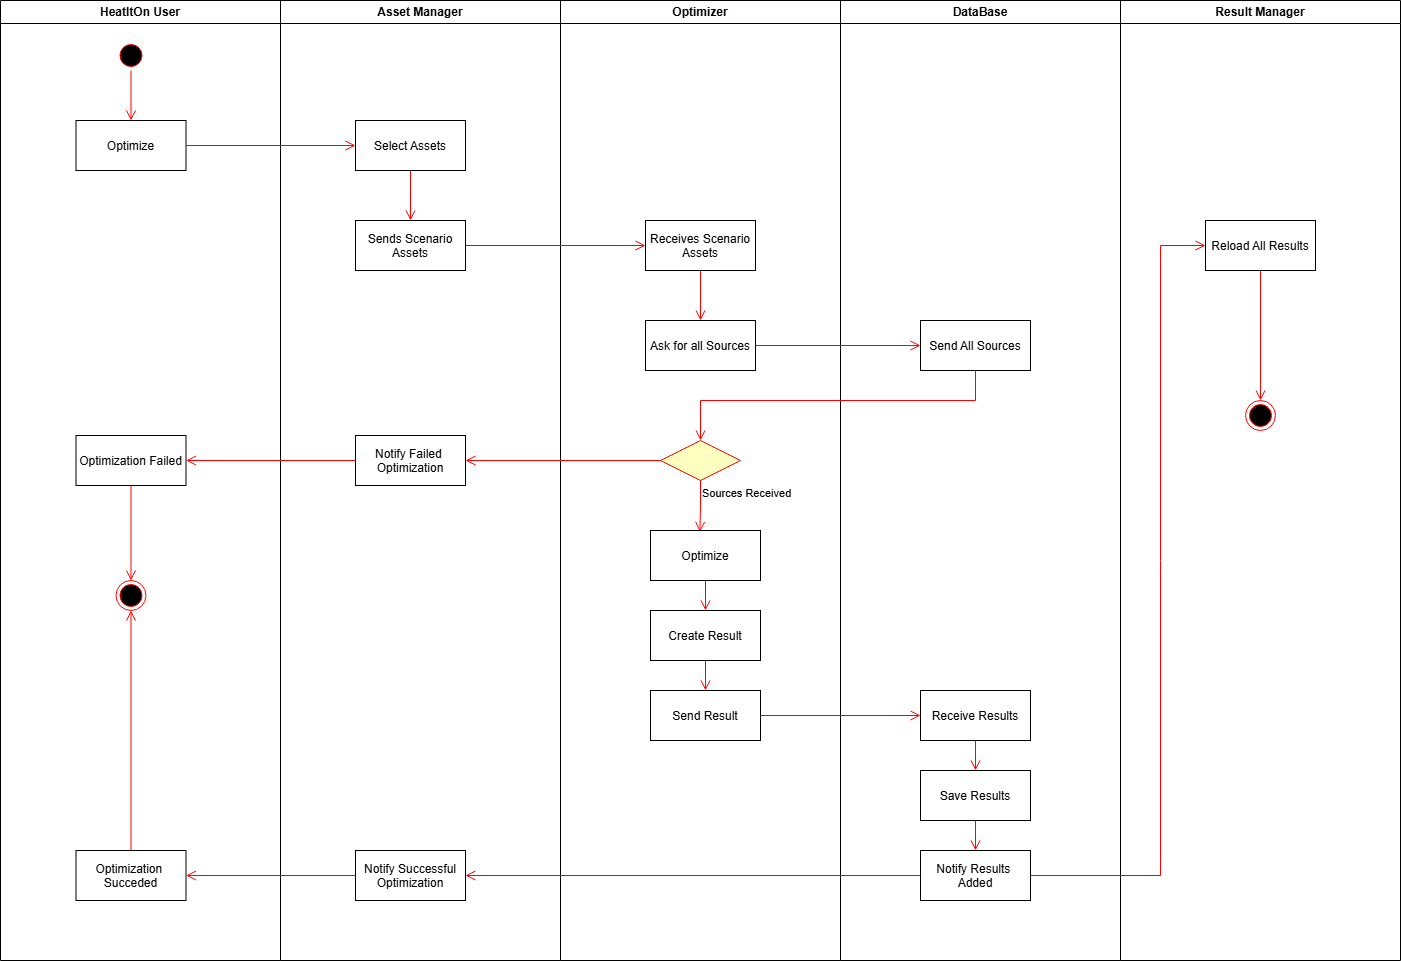
\includegraphics[width=0.9\textwidth]{Images/HeatItOn_activity_diagram_optimize.png} 
    \caption{Optimization Activity UML Diagram - Three parts and their actions for deleting Assets.}
    \label{fig:optimization_uml}
\end{figure}

The activity UML diagram (Figure~\ref{fig:optimization_uml}) depicts the optimization process.

First, the optimization starts with the user, using the Asset Manager UI, selecting Assets and starting the optimization process. The Asset Manager will send the selected Assets to the Optimization module, which after receiving them, will call from the Database all stored Sources up to that moment. If no Source is received it will prompt the Asset Manager to notify the user and end the activity. The Optimizer has no UI elements and is completely in the Backend. If it receives Sources, it will run the optimization algorithm, which will create a Result. The new Result is sent and stored in the Database that will notify both the Asset Manager(that in turn notifies the user) and the Result Manager that there is a new Result ready to be displayed, ending the activity.

This activity diagram proves its relevancy by demonstrating the optimization activity, which is the entire purpose of the system. While it is not enough for a full understanding of the optimization process, the diagram illustrates the different overall steps happening.

Optimization is the part that interacts with every module of the system. It uses directly or indirectly every implemented Manager, and all the activity diagrams(and all their depicted actions) are just helping the optimization process depicted here.

\subsection{UML Diagram - Sequence Diagram (Optimize)}

\begin{figure}[H]
    \centering
    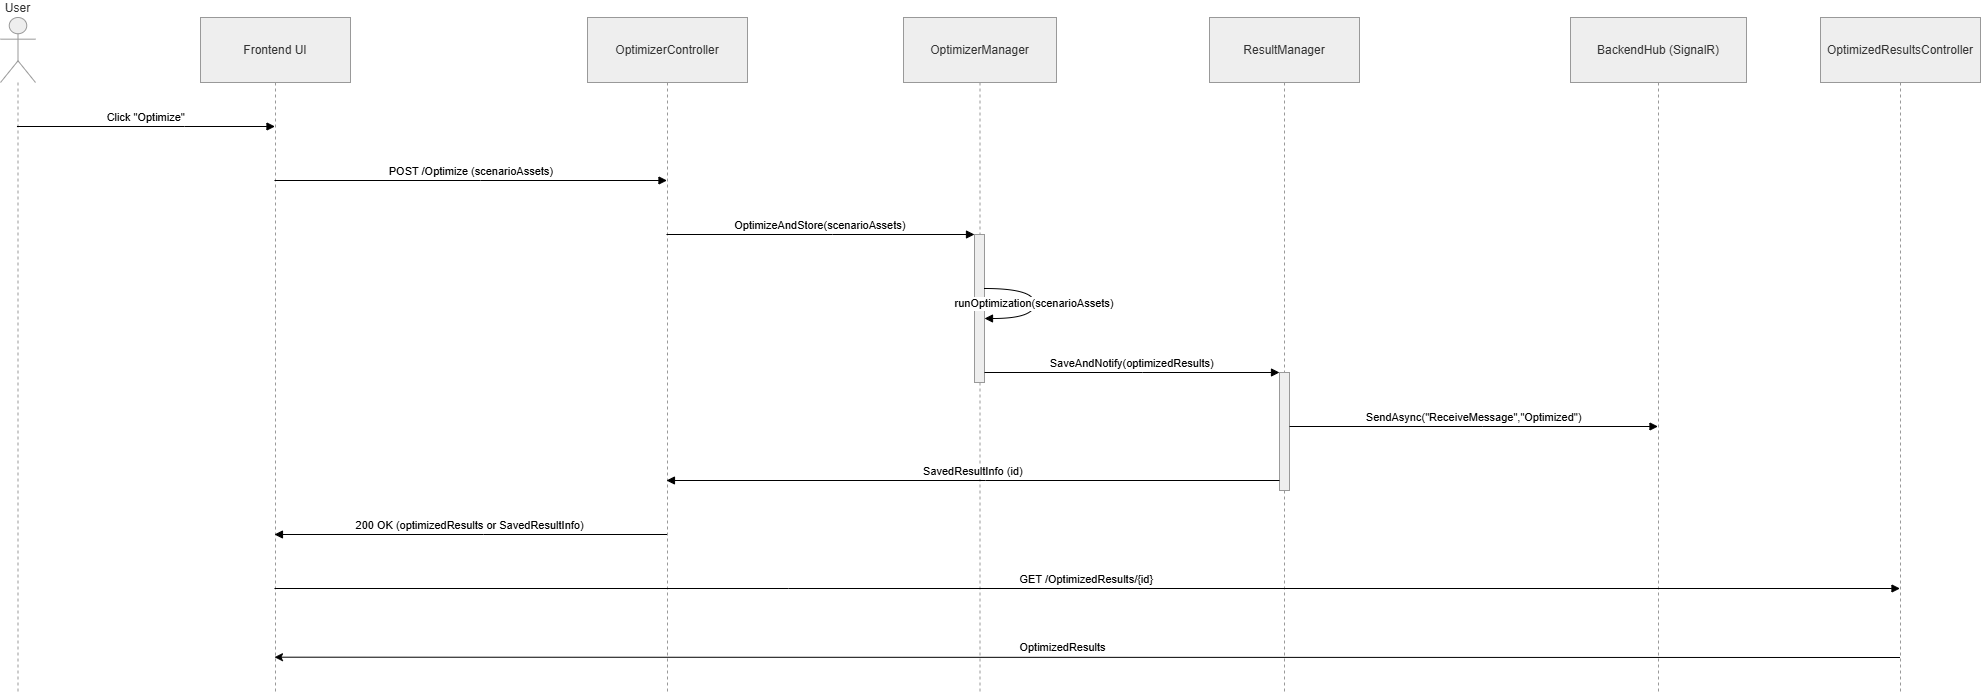
\includegraphics[width=0.9\textwidth]{Images/Sequence_diagram_optimize.drawio.png}
    \caption{Sequence UML diagram of optimization process}
    \label{fig:optimization_sequence}
\end{figure}

\hspace*{1cm}The sequence UML diagram (Figure~\ref{fig:optimization_sequence}) depicts the optimization process. The participants are: User, Frontend UI, `OptimizerController`, `OptimizerManager` (runs the algorithm), `ResultManager` (saves results and sends notifications), `BackendHub` (SignalR) and `OptimizedResultsController` (for later retrieval). The flow is: the user clicks Optimize in the frontend, the frontend sends the selected assets to `OptimizerController` with `POST /Optimize`, `OptimizerController` calls `OptimizerManager` to run the optimization, `OptimizerManager` produces an `OptimizedResults` object and gives it to `ResultManager` to save, `ResultManager` writes the result to the database and asynchronously notifies clients via `BackendHub.SendAsync("ReceiveMessage","Optimized")`, the controller returns either the full result or a small confirmation (`SavedResultInfo` with the new id) to the frontend, the frontend can then request the stored result with `GET /OptimizedResults/{id}` from `OptimizedResultsController` to display the full persisted data. If the optimizer cannot find required source data, it returns an error/notification back to the frontend and the activity ends with the user being informed. In the diagram the `OptimizerManager` and `ResultManager` are shown as manager boxes that group the backend logic (they represent the real services and saving/notification steps) so the sequence stays easy to read while matching the actual system behavior. 

This sequence diagram shows the main flow: how a user action becomes an optimized schedule and is delivered to the UI, connecting the user, backend computation, storage and real-time updates so the reader sees the end-to-end behavior without needing the algorithm details.

How this maps to the code:

\begin{itemize}
    \item The optimizer endpoint is in OptimizerController, the OptimizerController receives the POST /Optimize request.
    \item The optimization work runs in OptimizerService (this is the diagram’s OptimizerManager).
    \item Saving the results is done by OptimizedResultsService (the diagram’s ResultManager).
    \item Real-time notifications go through SignalR in BackendHub, controllers use IHubContext<BackendHub>.SendAsync to send messages.
    \item Fetching stored results is handled by OptimizedResultsController.
    \item The database model and migrations are in BackendDbContext.
    \item Centralized error handling (turning exceptions into HTTP responses) is implemented in ExceptionHandlingMiddleware.
\end{itemize}

\subsection{UML Diagram - Sequence Diagram (Refresh)}

\begin{figure}[H]
    \centering
    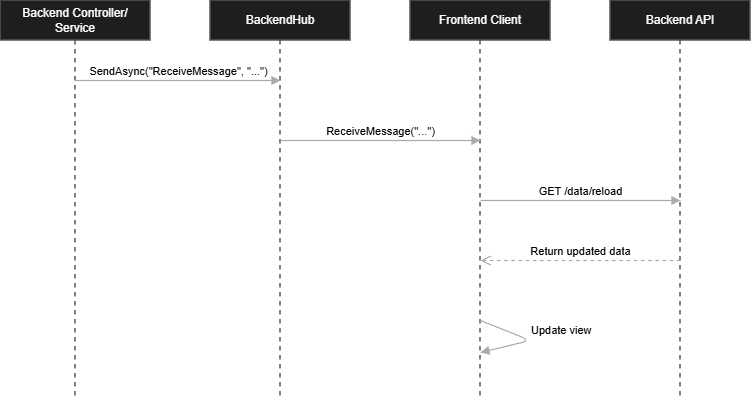
\includegraphics[width=0.9\textwidth]{Images/Sequence_diagram_refresh.png}
    \caption{Sequence UML diagram of refreshing process}
    \label{fig:refresh_sequence}
\end{figure}

\hspace*{1cm}The refresh sequence diagram is relevant because it shows how the frontend stays synchronized with changes made in the backend, which is an important part of the system’s behavior. It demonstrates the full update flow after a backend action has changed some data: the backend first sends a SignalR notification and then the frontend reacts by loading the latest data again. This makes the diagram useful because it explains how the user sees updated information without manually reloading the page and it also shows the difference between pushing a notification and pulling the new data. The diagram connects directly to the implemented solution in the codebase: controllers and services use `IHubContext<BackendHub>` to call `SendAsync(...)`, the frontend receives the `ReceiveMessage` event and then it requests the updated data from the backend through endpoints such as `OptimizedResultsController` or another reload request. In this way, the diagram reflects the real implementation and shows how real-time updates are handled in the system.
\section{System Technical Architecture}

\hspace*{1cm}For the system architecture, from a technical standpoint, C\# \cite{csharp} was chosen as the base technology stack. This was chosen as its .NET 9.0 version is suitable for the development of this system with its simplicity, the familiarity of the team and its object-oriented imperative style. Every other piece of technology is related to .NET and was chosen based on their respective compatibility with the language.

\subsection*{Technology Stack}

\hspace*{1cm}The first chosen piece was the Database that is running MySQL \cite{dubois2013mysql}. The role of the Database is to store the system data independently from other parts of the system(Backend and Frontend). It stores relevant user data, using models, like the Assets, Sources, Results of each generator and Results of optimization runs. The Database communicates with the Backend using MicrosoftEntityFramework. The Frontend cannot communicate directly with the Database, it must do it through the Backend. The Database allows data storage that is independent from runs. The system can work with multiple users at the same time or with one user in different runs, storing all the data in the Database, where it will remain until deletion.
 
The second chosen piece of technology stack is for the Frontend UI. For this AvaloniaUI was chosen for its good compatibility with .NET and modularity. Besides this, the Frontend is following the Model-View-ViewModel (MVVM) design pattern.

\subsection*{Layering}

\hspace*{1cm}The system is divided into three main parts, Frontend, Backend and the Database. Each serves a different role and, besides the Database, they are further separated for proper readability and modularity.

The Frontend, as stated earlier, follows the MVVM pattern. The Models, together with the Data (containing file I/O and clients) form the overall data and business layer. The View forms the presentation layer, containing all the UI elements. The ViewModel creates a connection layer between the two other parts. 

The Backend is following a .NET web application template. Its role is to create a connection between the Frontend and Database with an Application Programming Interface (API), and to handle overall business logic for the entire system. For modularity, this is achieved through serious layering. The Backend consists of six main parts. Controllers handle incoming/outgoing traffic to/from the Database and Frontend and will call the appropriate Services. Services contain all the business logic of the system(like optimization or add Asset). Both Controllers and Services inherit from two Interfaces, as they share similarities (like CRUD operations). The Data layer is composed of two other parts, Models(storing data models) and Data(storing DB Migrations and DB Context which is the main connection point to the DB). The presentation layer is completed by the last element, Hubs, which ensures real time communication with the Frontend application (instantly notifies to refresh the Frontend). Although the Backend is divided into many pieces, this was necessary for modularity, readability and because of complexity as well. This way each small section is responsible of one part, making replacement easier. In this solution, if one wants to hypothetically change the entire optimization algorithm, they only need to rework the Optimization Service, without having to touch any other parts.

\subsection*{Architectural Style}

\hspace*{1cm}The implementation follows multiple coding and design principles. The main set of principles that the project adheres to, is SOLID. This happens in both Frontend and Backend and is visible in many parts, like interfaces or being able to add new features without having to change code. SOLID principles help create an Object-Oriented design. But besides these, the project follows DRY (Do not Repeat Yourself), KISS  (Keep It Simple, Stupid), YAGNI (You Aren't Gonna Need It) and SoC (Separation of Concerns).

The technology stack, the layering and the architectural style used are all necessary for the proper running of the system. While the technology stack was kept simple by only using what was necessary for achieving requirements, the layering and style help build a good quality project that is easy to understand, change and complete. But extensive layering also helps following the style, by breaking up the large task into small sections creating a \textit{Divide et impera} style of development, making it easier to adhere to the principles.  


                             

\chapter[Implementation and Technical Realization]{Implementation and Technical Realization}             
\label{chap:implement}                                            
% -------------------------------------------------------------
% IMPLEMENTATION AND TECHNICAL REALIZATION
% -------------------------------------------------------------


\noindent HeatItOn is divided into three sections, and two versions. First there is the midterm evaluation demo version, and then there is the final version. We will go through both to see the first implementation and the improvements and changes that we made for the final version. 

\section{Frontend Implementation}

\hspace*{1cm}Our Frontend Implementation is desgined with the plant operators in mind, keeping it simple and user friendly. To achieve this, we started with a UI-sketch where we tried to come up with an easy to use and easy to understand concept, that we tried to achieve in our implementation.
 	
The application is split into three different tabs. The first one, that the user sees when they launch the application is the Assets tab. Here the user can manage and see all the existing assets \cite{projectassetsdata}, they can import or export assets as csv's or manually add/remove or edit specific assets one by one. This page also has three preset toggles(Scenario 1, Scenario 2 and Custom). As the Assets page is where the operator will start the optimization process, by selecting the asset combination they want to optimize with, the toggles merely select from the assets the ones that are in that scenario. If they wish to optimize for a new scenario, they can select the Custom toggle, allowing them to run the optimization process for any scenario. After selecting the desired assets the user has to click on the Optimize button that will start the optimization process for the selected assets. 
	
The list of assets is connected through the backend with the database, each modification being done live in the database. The optimization process from the backend is called from the frontend by clicking a button. The Assets tab will send the Optimization algorithm the assets selected to be optimized every time the button is clicked.
	
The second tab, the Results tab is where, once the user started an optimization, the result of that run will appear. On the left side, they can see and select out of a list of all results. When they select one result, the user can see the hourly result in a table format or view the data in different graphs. They can also export them into csv's. If the user would like to focus on a specific time period, not the entire optimiziation run, they can use a date-time picker to select from when to until when they want to see the result data, which will affect the result table and the graphs as well.
	
The tab loads all the optimization-results from the database using the backend services.
	
The third tab, Sources, is where the user will upload/export or even edit source data. On the left, you can see a list of uploaded csv's again. When the user selects one, they can also visualize the source data in a few simple charts or see the entire source data in a table. The cells of the table are modifiable so they can also edit the source data.
	
This tab uploads all sources directly to the database, using the backend services, while the csv file's are handled locally.
	
Our goal with each tab was acheaving an easily navigable and understandable UI, while giving all the necessary tools for the plant-operators/users for adequate management. Although we only received source data for four weeks and two asset scenarios, we tried to create a scalable, modular UI, that can handle dozens of assets and years worth of source data. As a side goal we also wanted to achieve a simple yet modern and visually appealing look.

\subsection{Midterm Version}

\hspace*{1cm}For the midterm demo, we prioritised usability over aspect. As this version was a mere proof of concept, and its goal was to plant a picture of our way of implementing it and to show what we think is possible, some aspects of the overall user experience was ignored so we can focus on actual functionality.

This means that the UI for this version has a very generic, template look. Buttons are rough and placed where we could fit them, while icons are uninteresting and unintuitive. A majorly different approach for displaying assets, results and sources was used in this version. Instead of the frontend lists updating to changes accordingly(like uploading csv's or generating results) in real time, we added a refresh button that, when clicked, reloads all the data from the database. This solution was a compromise made for this version, and eliminating it, a focuspoint for the final version.

The Assets tab was fully functional, and only needed some visual and aesthetic improvements (see Appendix \ref{appendix:figures}).



The Results tab in this version is defined by minimalistic graphs, that made it hard to visualize the results. Our three graphs(electricity use/production, heat production and CO2 production) were a good start but we realised we need a lot more for proper visualization. (see Appendix \ref{appendix:figures}).

The Sources tab functioned as expected but the possibility to edit the csv data was missing from this version.

Overall the demo was a very solid proof of concept that helped us learn what we were missing for the final version while also showing us the direction we are going.
	
\subsection{Final Version}
\hspace*{1cm}The final version focuses more on user experience with minor fuctionality improvementse when compared to the midterm implementation. The primary goal of this version was to improve usability, visual appearance, and introduce additional statistical aspects while maintaining a consistent and scalable structure. 

A significant improvement is the change from a manual data refresh system to a dynamic, responsive interface. In contrast to the midterm version, where a dedicated refresh button was required to update data, the final implementation ensures that all lists and views update automatically in response to changes in the database. This enhancement improves workflow efficiency and eliminates unnecessary user interaction.

The visual design of the interface has been improved. The final version adopts a modern, structured design with consistent colors, clearer text formating, and improved spacing. Asset cards have been redesigned to display key information in a meaningful and readable format, including maximum heat, production cost, CO\textsubscript{2} emissions, and electricity generation/consumption. Additionally, asset categories such as gas, oil, electric, and motor are visually distinguished through icons and labels, allowing for faster recognition and comparison.

The scenario selection system has been refined and better integrated into the workflow. Instead of simple toggles, the final version introduces clearly defined scenario panels with descriptive labels such as “Peak Load,” “Eco Mode,” and “Custom Configure.” Each scenario communicates its purpose more effectively, enabling more intuitive decision-making. Furthermore, visual indicators highlight selected assets within each scenario, improving clarity during configuration.

Additional controls have been add, including a “Manager” and an “Optimize” button. The Manager section serves as a centralized interface for creating, importing, and exporting assets. These improvements lead to a clearer workflow, guiding the user from setup to execution in a more structured way.

The Results tab has undergone major enhancements in both data presentation and analytical depth. A summary dashboard has been introduced at the top of the page, presenting key performance indicators such as total heat production, net electricity balance, total CO\textsubscript{2} emissions, and total production cost. These aggregated metrics provide immediate insight into optimization outcomes without requiring detailed inspection of raw data.

The data display has also been improved with better formatting, clearer column labeling, and pagination support for large datasets. The addition of pagination ensures that even large datasets remain readable and manageable.

The charting system represents one of the most significant functional improvements. While the midterm version included only basic visualizations, the final version introduces a comprehensive set of charts:
\begin{itemize}
\item A stacked area chart showing heat production per asset over time, including a total heat overlay
\item A production cost per hour chart, allowing detailed financial analysis
\item A generator share pie chart, illustrating the contribution of each asset within a selected time range
\item An electricity usage and generation chart, displaying hourly electricity balance in MWh
\end{itemize}

These visualizations provide a deeper understanding of system behavior and allow users to analyze performance trends, cost distribution, and resource utilization more effectively. Interactivity elements, such as tooltips and time-range filtering, further enhance data exploration.
The date and time filtering functionality has been refined, with a more structured input system for selecting precise time intervals. Filtering affects both tabular and graphical outputs, ensuring consistency across all displayed data.

The Sources tab has also been expanded with important new functionality. Unlike the midterm version, the final implementation allows direct editing of source data within the table. This feature enables on-the-fly adjustments without requiring external file modification. The table design has been improved for clarity, and pagination has been introduced to handle large datasets efficiently.
File management capabilities have been enhanced, including clearer separation between uploaded files and active data views. Import and export functions remain available but are now better integrated into the interface.

Overall, the final version achieves a significantly higher level of usability, clarity, and analytical capability. The transition from a proof-of-concept interface to a polished, production-oriented design is evident across all tabs. The system now provides a comprehensive toolset for asset management, optimization execution, and result analysis, while maintaining a scalable and user-centered design approach.

\section{Backend Implementation}
\subsection{Midterm Version}

\hspace*{1cm}The backend is implemented using ASP.NET Core 9.0 and follows a layered architectural design that emphasizes modularity, scalability, and separation of concerns. The structure consists of Controllers, Services, Interfaces, Models, and a Data layer, each responsible for a distinct part of the system functionality.


\textbf{Architecture and Main Components}

\begin{figure}[H]
\centering
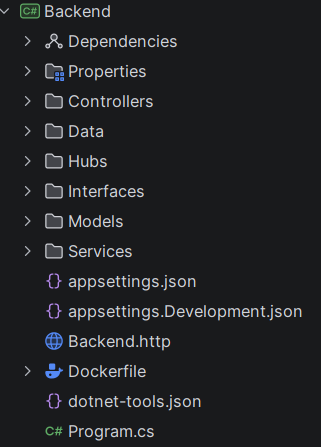
\includegraphics[width=0.6\textwidth]{Images/backend-file-structure.png}
\caption{Backend file structure showing the organization of controllers, services, interfaces, models, and data components.}
\label{fig:backend-structure}
\end{figure}

The backend is organized into clearly defined layers:

\begin{itemize}
    \item \textbf{Controllers}: Provide RESTful API endpoints and act as the entry point for client requests. Controllers are responsible for handling HTTP requests, binding input parameters, and returning appropriate responses.
    
    \item \textbf{Services}: Implement the core business logic. Each service corresponds to a domain entity, such as assets, source data, and optimization results. Services coordinate data processing and communicate with the persistence layer.
    
    \item \textbf{Models}: Represent domain entities and map directly to database tables. Examples include \texttt{Asset}, \texttt{Source}, \texttt{Result}, \texttt{ResultList}, and \texttt{OptimizedResults}.
    
    \item \textbf{Data Layer}: Contains the Entity Framework database context (\texttt{BackendDbContext}) and migration files. This layer manages communication with the MySQL database.
\end{itemize}

This architecture ensures that responsibilities are clearly separated, enabling easier maintenance and extensibility.


\textbf{API and Controller Design}

During the midterm the backend exposed basic REST endpoints (CRUD) implemented ad-hoc, these were formalized in the final version through generic controller/service interfaces (see the \textbf{Final Version} subsection).

All controller actions are implemented asynchronously using \texttt{Task<IActionResult>}, allowing efficient handling of concurrent requests. Controllers delegate processing tasks to the service layer, keeping the API layer thin and focused on HTTP concerns.


\textbf{Business Logic Handling}

All business logic is implemented within the service layer, which acts as the core processing unit of the backend. Each service implements the generic \texttt{IService<T>} interface, providing consistent operations across all entities.

Specialized services, such as the \texttt{OptimizerService}, encapsulate domain-specific logic related to heat production optimization. This includes processing input data, calculating results, and coordinating interactions between assets, source data, and result data.

The separation of business logic from controllers improves maintainability and enables independent testing of core functionality.


\textbf{Data Processing and Validation}

Data processing is primarily handled within the service layer. Incoming data from API requests is validated before being persisted or processed further. Validation mechanisms include:

\begin{itemize}
    \item Strongly typed C\# models for structured data representation
    \item Parameter binding and validation features provided by ASP.NET Core
    \item Logical validation rules implemented within service methods
\end{itemize}

This approach ensures that invalid or inconsistent data is prevented from entering the system and maintains overall data integrity.


\textbf{Database Communication}

The backend communicates with the MySQL database using Entity Framework. The \texttt{BackendDbContext} manages entity tracking, query execution, and persistence.

\begin{itemize}
    \item Models are mapped directly to database tables
    \item LINQ is used for querying and manipulating data
    \item Asynchronous database operations improve performance and scalability
\end{itemize}

Services interact with the database context to perform all data operations, ensuring controlled access to the persistence layer and preventing direct database access from controllers.


\textbf{System Behavior Support}

The backend supports the required system behavior by coordinating interactions between different system modules. Controllers expose endpoints for managing assets, source data, and optimization results, while services execute the corresponding logic.

The inclusion of a dedicated optimization service enables the processing of time-series data for heat demand and electricity prices, supporting the generation of optimized production schedules.


\textbf{Deployment Considerations}

The backend is deployed using Docker, which provides a consistent and isolated runtime environment. Containerization ensures that dependencies, configurations, and runtime settings are standardized across development and production environments.

This approach improves portability, simplifies deployment, and enhances the reliability of the backend infrastructure.


Overall, the backend implementation follows best practices for modern web application development, emphasizing modularity, scalability, and maintainability. The layered architecture ensures that the system can effectively support the required functionality while remaining adaptable to future enhancements.

\subsection{Final Version}
\hspace*{1cm}The final backend version extends the original layered ASP.NET Core architecture with additional runtime functionality and tighter system integration. We introduced two supporting components: a centralized exception-handling middleware and interface-based service contracts that define abstraction boundaries between controllers and services.

These additions work together with the existing layers as follows: controllers accept HTTP requests and delegate work to services; services implement business logic and interact with the data layer (EF `BackendDbContext`); both controllers and services rely on the `Interfaces` abstraction and dependency injection; the `ExceptionHandlingMiddleware` sits early in the request pipeline, catching exceptions from controllers and services, logging them, mapping domain errors to HTTP status codes, and returning compact JSON error responses. As a result, many local try/catch blocks were removed and method implementations became easily readable.

\begin{itemize}
    \item \textbf{Exception handling}: Centralized in \texttt{ExceptionHandlingMiddleware}. It intercepts exceptions thrown by controllers and services, logs them, maps domain errors to appropriate HTTP status codes, and returns a compact JSON payload (for example \texttt{\{}\texttt{"error":} \texttt{"<message>",}\texttt{"stackTrace":}\texttt{"<stackTrace>"}\texttt{\}}) with \texttt{Content-Type:}\texttt{application/json}. This provides consistent, machine-readable error responses for clients and prevents raw error details from leaking.
    \item \textbf{Interfaces}: Provide clear abstraction boundaries for controllers and services \\ (e.g., \texttt{IController <TCreate,TUpdate>}, \texttt{IService<T>}). Using interfaces enables dependency injection, easier unit testing, and consistent error-typing so the middleware can map domain exceptions to appropriate HTTP responses.
    \begin{itemize}
        \item The generic controller interface formalizes standard CRUD operations used across controllers:
        \begin{itemize}
            \item \texttt{List()} for retrieving collections of entities
            \item \texttt{Get(int id)} for retrieving a single entity
            \item \texttt{Post(TCreate model)} for creating new entries
            \item \texttt{Put(int id, TUpdate model)} for updating existing entries
            \item \texttt{Delete(int id)} for removing entries
        \end{itemize}
    \end{itemize}
    \item \textbf{Controllers}: Handle request/response concerns and remain thin — delegating business rules to services and relying on interfaces for testability, validate inputs.
    \item \textbf{Services}: Contain core business logic, interact with the data layer, and throw well-defined domain exceptions when needed. They do not implement HTTP concerns or repeated try/catch logic anymore.
    \item \textbf{Data layer}: The Entity Framework \texttt{BackendDbContext} and related repositories/models remain responsible for persistence and are used by services through interface-driven abstractions.
\end{itemize}

\section{Data Management}
\subsection{Midterm Version}
Data management is implemented using a relational database approach supported by MySQL, combined with an object-relational mapping layer provided by Entity Framework.

\textbf{Data Structure}

\begin{figure}[H]
\centering
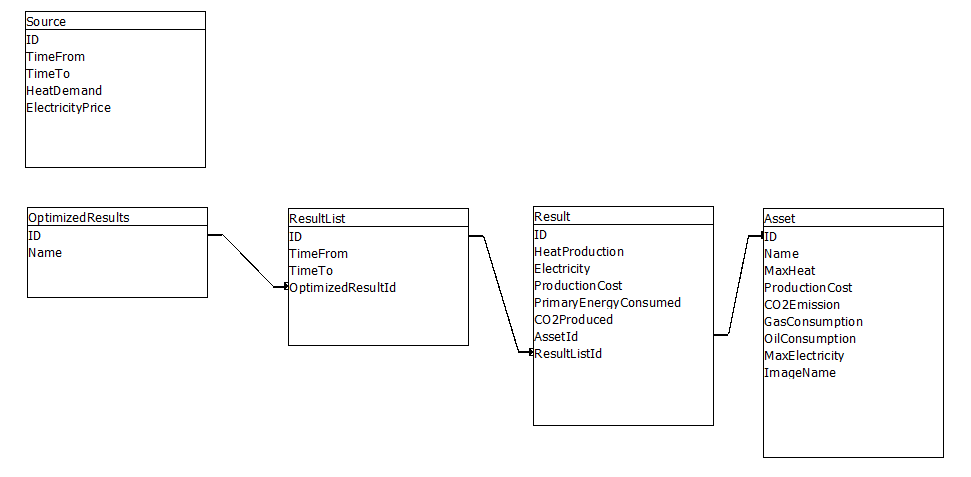
\includegraphics[width=1\textwidth]{Images/db-relations.png}
\caption{Database schema illustrating the relationships between Source, OptimizedResults, ResultList, Result, and Asset tables.}
\label{fig:db-schema}
\end{figure}

The data model is organized into five primary tables: Source, OptimizedResults, ResultList, Result, and Asset, each representing a distinct aspect of the system domain.
\begin{itemize}
\item The Source table stores time-based input data, including HeatDemand, and ElectricityPrice. This structure supports time-series data used for optimization processes.
\item The OptimizedResults table represents a container for optimization runs during the selected time period. 
\item The ResultList table links individual time intervals to a specific optimization result through the foreign key OptimizedResultId. Each entry contains results for separate assets within an hourly time frame, with attributes such as TimeFrom and TimeTo defining the interval. 
\item The Result table contains detailed output data generated by the optimization process. Attributes include HeatProduction, Electricity, ProductionCost, PrimaryEnergyConsumed, and CO2Produced. This table also includes foreign keys AssetId and ResultListId, establishing relationships with both Asset and ResultList. It stores the specific performance metrics for one asset in one hour.
\item The Asset table defines the characteristics of generators or boilers, including MaxHeat, ProductionCost, CO2Emission, GasConsumption, OilConsumption, MaxElectricity, and ImageName.
\end{itemize}

The relationships between these tables follow a hierarchical structure:
\begin{itemize}
\item One OptimizedResults entity relates to multiple ResultList entries.
\item One ResultList entry relates to multiple Result records.
\item Each Result references a single Asset.
\end{itemize}

Primary keys and foreign keys ensure referential integrity across all tables. For example, Result.AssetId must correspond to a valid entry in the Asset table, and ResultList.OptimizedResultId must reference an existing optimization result.

\textbf{Integration with Backend}

The data structure integrates directly with the backend through Entity Framework. Each database table is mapped to a corresponding C\# model, enabling seamless interaction between the application logic and the database layer. Entity Framework provides abstraction over raw SQL queries, allowing developers to interact with the database using LINQ queries and strongly typed objects. The DbContext component manages database connections, entity tracking, and query execution, ensuring consistent data access patterns across the application. Migration tools within Entity Framework support schema evolution, allowing controlled updates to the database structure while maintaining data integrity.

\textbf{Data Management Environment}

The database is deployed using Docker, ensuring a consistent and reproducible environment. The use of Docker also facilitates easy deployment, testing, and version control of the data management infrastructure.

Overall, the data management approach combines a well-defined relational schema, validation mechanisms, and seamless backend integration to ensure reliability, scalability, and maintainability of the system.

\subsection{Final Version}

\hspace*{1cm}The recent database updates were minor and mainly aimed at improving data quality. We added and refined several model-level validation rules using data-annotation attributes (such as Required, Range, and MaxLength) to prevent invalid or inconsistent values from being saved. We also introduced a unique constraint for the Source entity in the DbContext configuration to avoid creating duplicate entries. These changes strengthen validation and consistency across the system without altering the overall database structure.
                             

\chapter[Discussion and Reflection]{Discussion and Reflection}             
\label{chap:reflect}                                            
% -------------------------------------------------------------
% DISCUSSION AND REFLECTION
% -------------------------------------------------------------
\section{Discussion and Reflection}
% -------------------------------------------------------------
% DISCUSSION AND REFLECTION
% -------------------------------------------------------------
\hspace*{1cm} This chapter discusses the software engineering practices and processes adopted throughout the project. It also contains potential future work that could further improve the product. 

\section{Scrum}
\hspace*{1cm} ``Scrum is a lightweight framework that helps people, teams and organizations generate value through adaptive solutions for complex problems.''\cite{scrumguide} One of Scrum's core principles is the division of work into sprints, which usually last one or two weeks. ``All the work necessary to achieve the Product Goal, including Sprint Planning, Daily Scrums, Sprint Review, and Sprint Retrospective, happen within Sprints.''\cite{scrumguide}

\begin{itemize}
    \item Sprint Planning took place on either Fridays or Mondays, depending on the team's availability. During these sessions, pre-planned tasks were moved from the backlog to the current sprint in Jira, where they were assigned to team members and estimated using story points. This practice led to better team organization, improved communication, and a clearer structure that kept the workflow predictable. 
    \item Daily Scrums took place on Mondays, Wednesdays, and Fridays. During these short 10--15 minute sessions, each team member addressed their accomplishments, struggles, and future plans.
    \item Sprint Review took place at the end of each sprint. Each team member summarized their individual participation, struggles, and opinions on the sprint. Following that, the Scrum Master provided an overall summary of the sprint's accomplishments while assessing completed and incomplete tasks. The session concluded with a review of the sprint as a whole.
    \item Sprint Retrospective took place immediately after the Sprint Review. Using a dedicated document in Jira, the team filled out a simple table with three columns: Start Doing, Stop Doing, and Keep Doing. Each team member added their thoughts to each column, after which the entries were discussed together as a group. 
\end{itemize}

\section{Requirements Engineering}
\hspace*{1cm} ``Requirements engineering is the process of understanding and defining what services are required from the system and identifying the constraints on the system's operation and development.''\cite{scrumguide} Practises used during this project:
\begin{itemize}
    \item User stories - Kept focus on problems from user perspective
    \item Product Backlog - Provided a full and organised list of all tasks
    \item Functional requirements - Ensured all members of team understood what the software is supposed to do
    \item Non-functional requirements - Ensured all members of team understood the quality standard the software needed to meet
    \item Story points - Estimated the effort for all the tasks
    \item Sprint backlog - Helped the team stay focused on tasks chosen from the backlog for the current sprint
    \item Reviews with the team - Allowed each member to validate certain tasks helping to reveal and prevent mistakes and errors
    \item Definition of Done - Determined what finished task mean (code, testing, reviews)
\end{itemize}
\hspace*{1cm} In the future, all of these practices will be used again. User stories will be written in more detail, the product backlog will be prepared more thoroughly at the beginning of the project, and reviews will be taken more seriously.

\section{Refactoring}
\hspace*{1cm} Throughout the project, several refactoring improvements were made to keep the codebase clean and maintainable. CSV-related functionality was combined into a single unified class to reduce duplication. A centralized error handler was introduced, removing repetitive try-catch blocks from services and controllers. Data annotations in the models were expanded for better input validation, and interfaces were added to improve code structure. Unused imports were removed, formatting was cleaned up, and inheritance structures were reviewed and adjusted where needed.\section{Code review}
\hspace*{1cm} During this project, two reviewers were assigned to every task in Jira and GitHub. Both had to either approve or request changes, and all issues had to be resolved before merging the work into the main branch. This practice helped improve overall code quality and catch bugs early in the process.

However, this practice came with some challenges. Some reviews were delayed or not done properly enough, which occasionally led to mistakes slipping through. The team addressed these issues to prevent them from happening in the future.

\section{Testing}
\hspace*{1cm} During the project, unit tests were written for every task that involved business logic. Testing was part of the Definition of Done, meaning tasks could not go for review until the necessary tests were written.

Manual end-to-end testing was conducted to ensure the application ran and behaved as expected. For tasks involving the database, Postman was used to test every endpoint after new code was added or modified.

As unit testing was a relatively new practice for most team members, it was occasionally forgotten and done retrospectively, or not completed properly due to lack of experience.
                             

\chapter[Conclusion]{Conclusion}             
\label{chap:conclusion}                                            
\section{Conclusion}
\hspace*{1cm} HeatItOn is a utility in the city of Heatington that supplies heat to 
approximately 1,600 buildings through a centralized district heating network. Prior to 
this project, heat production was planned manually, making it difficult to consistently 
select the most efficient combination of production units. The goal was to replace this 
manual process with an automated optimization system capable of generating heat 
production schedules that consistently meet heat demand while minimizing operational 
costs.

\hspace*{1cm} The system was built around five core modules: the Optimizer, Data 
Visualization, Asset Manager, Source Data Manager, and Result Data Manager. The 
architecture followed a clear separation between the Frontend, Backend, and Database 
layers.

\hspace*{1cm} Both required scenarios were successfully implemented. Scenario 1 covered 
a heat-only network, where the system prioritized cheaper units and handled maintenance 
scheduling. Scenario 2 introduced electricity production, where the optimizer calculated 
net production costs on an hourly basis to determine when to sell or consume electricity. 
A custom scenario was also implemented, giving users control over which assets are 
included in the optimization.

\hspace*{1cm} The final product successfully addressed the original problem statement. 
The system is able to automatically generate optimized heat production schedules that 
meet the heat demand of Heatington while minimizing operational costs, replacing the 
previous manual planning process entirely. Operators can now manage assets, import 
source data, run the optimizer, and view the results through a single integrated 
application.

\hspace*{1cm} Looking ahead, the system could be further extended in several ways. 
Integrating live electricity prices from Energinet.dk would allow the optimizer to react 
to real-time market data. The ability to enable or disable individual units directly from 
the user interface would give operators greater flexibility during optimization. In future 
development, the team would also focus on improving test coverage, refining the user 
interface based on user feedback, and expanding the system to support additional heating 
scenarios.
                             

% -------------------------------------------------------------
%AI USAGE
% -------------------------------------------------------------            
\chapter[AI Usage]{AI Usage}             
\label{chap:ai}                                            
% --------------------------------------------------------
% AI USAGE
% --------------------------------------------------------
\noindent Throughout the project, the team incorporated AI across multiple stages to assist with various tasks. Importantly, AI was never used as a replacement for human effort or core decision-making. Instead, it served exclusively as a supplementary tool to streamline team workflows and optimize overall time management. 

\subsection*{Some of the examples using AI in this project:}
\begin{itemize}
    \item \textbf{Architectural Brainstorming:} In the early planning stages, AI was leveraged to help generate ideas for potential design patterns and library integrations. Team then carefully weighed these options against established non-functional requirements before finalizing the architecture. 
    \item \textbf{Debugging Assistance:} Dealing with undocumented Avalonia UI errors or sudden backend disconnects sometimes meant untangling obscure error codes. AI was used as a supplementary tool to quickly parse these codes, though diagnosing the root cause within our specific architecture and developing the actual fixes remained a manual team effort. 
    \item \textbf{Formatting and Documentation:} To streamline team workflow, it was decided to outsource repetitive formatting tasks to AI tools. This included generating UML diagram sketches from our existing C\# codebase to then format those in a specific editor and resolving some of tricky LaTeX compilation errors in the report, which saved valuable time without affecting the design or logic of the core system. 
    \item \textbf{UI/UX Inspiration:} Various stylistic directions were explored for project logos and interface by generating mood boards with AI image tools. Even though the final application relies exclusively on original assets, these early visualizations helped steer overall design choices. 
    \item \textbf{Code Review and Refactoring:} During the refactoring phase, AI acted as an extra set of eyes to catch missed references. When renaming methods within optimization modules, for instance, it helped verify that all old instances were properly updated, effectively reducing minor human errors without altering the underlying code logic.
\end{itemize}
                             

% -------------------------------------------------------------
% APPENDIX
% -------------------------------------------------------------
\appendix                                                     
% -------------------------------------------------------------
% APPENDICES
% -------------------------------------------------------------
\section{Appendices}

\begin{figure}[h]
    \centering
    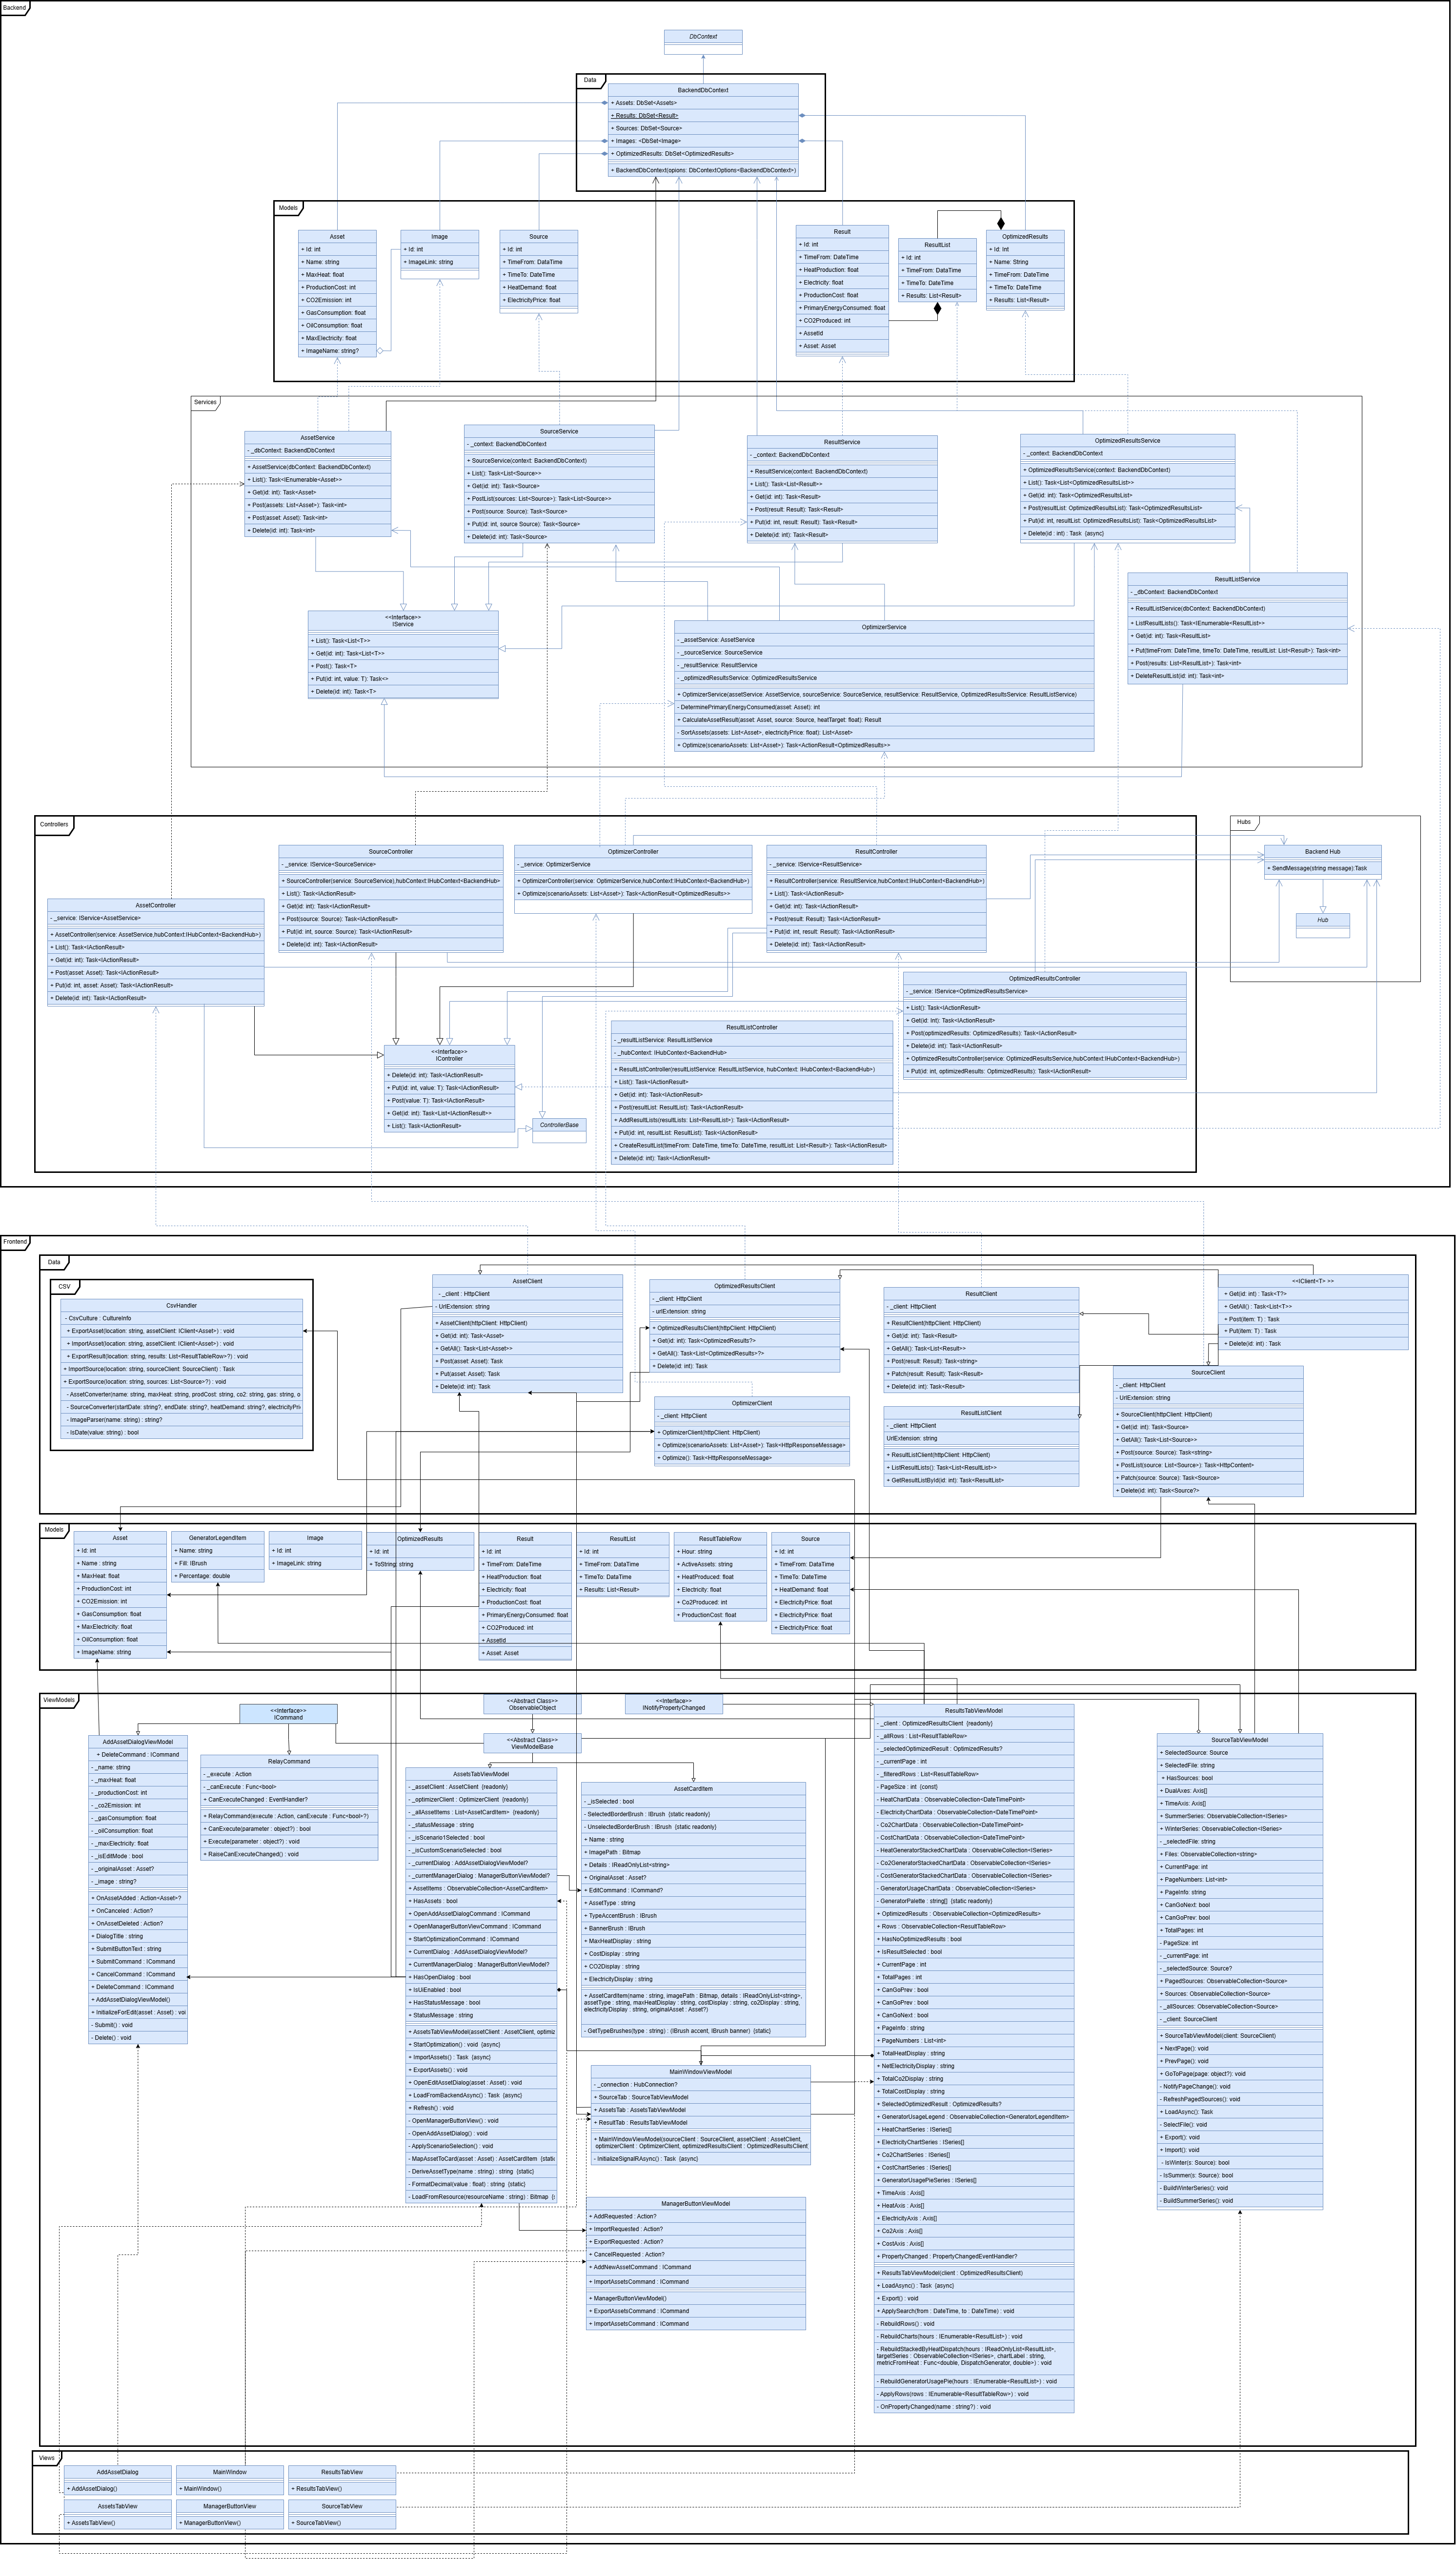
\includegraphics[width=0.9\textwidth]{Images/full_class_uml.png} 
    \caption{Package UML Diagram - Five main packages of the system.}
    \label{fig:package_uml}
\end{figure}
                                 


\end{document}
